\documentclass[12pt]{article}
\usepackage[utf8]{inputenc}
\usepackage{graphicx}
\usepackage{wrapfig}
\usepackage{tabularx}
\usepackage{lipsum}
\usepackage{pgfgantt}
\usepackage{indentfirst}
\linespread{1.5}
\usepackage{geometry}
\usepackage{minted}
\usepackage{float} 
\usepackage{times}
\geometry{left = 1.5in,
            right =1in,
            top=1in,
            bottom=1in}
\usepackage{amsmath}
\usepackage{anyfontsize}
\usepackage[style=ieee]{biblatex}
\addbibresource{bibliography.bib}
\pagenumbering{gobble} 
\setlength{\parindent}{0pt}

\begin{document}

\begin{titlepage}
	\begin{center}
	
	\large%14pt
	A Minor Project Final Report on
	
	\huge %24pt
	\textbf{Presence: Automated Attendance System}

	\vfill
	
	\large %14pt
	Submitted in Partial Fulfillment of the \\ 
	Requirements for the Degree of \\ 
	\textbf {Bachelor of Engineering in Software Engineering} \\
	under Pokhara University
	
	\vfill
	
	Submitted by: \\ 
	\textbf {Rupesh Budhathoki, 191721} \\
	\textbf {Apsara Bishwokarma, 191704} \\
	\textbf {Sampada Kharel, 191723} \\
	\textbf {Sudarshan Kshetri, 191729} \\
 
	\vfill
	
	Under the supervision of: \\
	\textbf {Yogesh Deo}
	
	\vfill
	
	Date: \\
	\textbf {27 Sept 2023}
	
	\vfill
	
	\end{center}
	
	\begin{wrapfigure}{L}{0.2\textwidth}
	\centering
	
\includegraphics[width=0.2\textwidth]{figures/college-logo.png}
	\end{wrapfigure}
	
	\fontfamily{phv}\selectfont
	
	\textbf {Department of Software Engineering}  
	
	% \Large %17pt
        \LARGE %21pt
	\textbf {NEPAL COLLEGE OF} 
	
	\LARGE %21pt
	\textbf {\underline {INFORMATION TECHNOLOGY} }
	
	\small %11 pt
	Balkumari, Lalitpur, Nepal
	
	
\end{titlepage}

\newpage
\pagenumbering{Roman}
\setcounter{page}{1}
\addcontentsline{toc}{section}

\section{Acknowledgement}
We would like to express our gratitude to the many individuals who played a vital role in making the 
"Automated Face Attendance System" project a reality. Their support and guidance were crucial throughout the project, and we are sincerely thankful for their contributions.\\

We extend our special thanks to Mr.Birendra Bista, the Head of the Department of Software Engineering, for his invaluable guidance and technical support. Also our professor Dr. Roshan Chitrakar, for valuable suggestions, attention and time for our project. \\

 We also appreciate our supervisor Yogesh Deo, for constant motivation and support during the course of our work throughout the semester which helped our project to grow and foster to a certain level we didn’t think of reaching in such a short period.  We truly appreciate and value his esteemed guidance and encouragement from the beginning to the end of this project.\\ 

Above all, we would like to thank our friends whose direct and indirect support helped us to complete our project on time. This project would have been impossible without their moral support.
\\
\\
\newpage



\section{Abstract}
The "Presence" project is an innovative approach to attendance tracking in college classrooms. With the help of automation and data analysis, the system aims to provide a more efficient and accurate way of keeping track of student attendance while also providing valuable insights into student behavior and academic performance. The system uses cameras to detect when students enter and leave the classroom. The data collected is then analyzed to provide a real-time attendance report that instructors can access from their devices. This eliminates the need for manual attendance-taking and reduces the potential for errors or inaccuracies. In addition to real-time attendance tracking, the system also provides detailed reports on student attendance patterns, subject preferences, and behavior in class. By analyzing this data, instructors and administrators can identify students who may be struggling with attendance or academic performance and take proactive steps to address these issues. They can also identify trends and patterns in attendance that can inform decisions about course scheduling and curriculum design.\\

The "Presence" project is a valuable tool for both students and faculty. For students, it provides a streamlined attendance tracking process that eliminates the need for manual sign-ins and helps ensure that they are meeting attendance requirements. For faculty, it provides real-time insights into student attendance and behavior that can inform teaching strategies and improve academic outcomes.\\ 

\textbf{Keywords}--
\textit{ automated attendance system, data analysis, college classrooms, attendance tracking, attendance report, academic performance, attendance patterns, subject preferences, student behavior, teaching strategies, curriculum design }\\\\
\newpage

\newpage
\tableofcontents
\newpage
\listoffigures
\newpage
\listoftables
\newpage

\section{Introduction}
\pagenumbering{arabic}
% In today's technology-driven era, the trend is to switch from traditional systems to fast, smart, and interactive systems that can be linked to web applications, enabling users to access the system from anywhere at any time. In academic settings, regular attendance is crucial for students to acquire knowledge, participate in class discussions, and engage with their peers. However, traditional methods of taking attendance, such as calling out names or manually signing in, can be tedious, prone to errors, and inefficient.\\

To address these challenges, we propose the design and implementation of a face detection and recognition system called "Presence." The "Presence" system is an automated attendance system that utilizes facial recognition technology to identify and mark the attendance of students attending a lecture in a classroom. By automating the attendance process, "Presence" aims to save time for instructors, reduce errors, and provide a more accurate and efficient way to monitor student attendance.\\

The "Presence" system is an advanced and sophisticated system that uses a camera to detect the faces of students entering and leaving the classroom. The system will be designed to recognize individual faces, match them with the database of registered students, and mark their attendance automatically. The data collected by the system will be stored securely and can be accessed through a web application by instructors, students, and authorized personnel.\\

In addition to recording attendance, the "Presence" system will provide valuable insights into attendance patterns, such as how often a student attends a particular class or how long they stay in the classroom. This data can be analyzed to identify trends and patterns in student behavior, which can be used to make informed decisions about how to improve learning outcomes. \\

\subsection{Motivation/Problem Statement}
In today's technology-driven era, the trend is to switch from traditional systems to fast, smart, and interactive systems that can be linked to web applications, enabling users to access the system from anywhere at any time. In academic settings, regular attendance is crucial for students to acquire knowledge, participate in class discussions, and engage with their peers. However, traditional methods of taking attendance, such as calling out names or manually signing in, can be tedious, prone to errors, and inefficient.\\

The "Presence" project is developed to address the challenges associated with manual attendance-taking in college classrooms. Traditional methods of attendance tracking, such as paper sign-ins or roll calls, are time-consuming, prone to errors, and may not provide accurate or timely data for instructors and administrators. Additionally, manual attendance-taking does not provide insights into student behavior or attendance patterns, which can be valuable for improving academic outcomes and making data-driven decisions.\\

\subsection{Project Objectives}
To address these challenges, developed a face detection and recognition system called "Presence." The "Presence" system is an automated attendance system that utilizes facial recognition technology to identify and mark the attendance of students attending a lecture in a classroom. By automating the attendance process, "Presence" aims to save time for instructors, reduce errors, and provide a more accurate and efficient way to monitor student attendance.\\

The project had put forward the following objectives:

\begin{itemize}
	\item To automate attendance system for college classrooms
	\item To provide insights into attendance patterns and behavior.
        \item To support data-driven decision-making for improved student success.
  
\end{itemize}\\


\subsection{Significance of the study}
The "Presence" project holds significant importance as it introduces an automated attendance system that addresses the limitations of manual methods. It streamlines attendance tracking, provides real-time reports, and offers insights into attendance patterns and student behavior. This empowers educators to make data-driven decisions, optimize instructional practices, and enhance student success in college classrooms.\\

\newpage

% \section{Scope and Limitation}
% The scope of the "Presence" project is wide-ranging and encompasses various aspects of attendance tracking and data analysis in college classrooms. It will be designed to accommodate multiple subjects and courses, providing flexibility for instructors and students. The system's scope also extends to generating comprehensive attendance reports and analysis, enabling instructors and administrators to gain valuable insights into attendance patterns, subject preferences, and student behavior. Additionally, the project has the potential for future expansion and integration with other educational technologies, further enhancing its scope and usability.
\\
% \break
% The following are the limitations of the project that are realized:
\begin{itemize}
 	
        \item The system may not work accurately in low lighting or poor camera quality environments.
        \item The system will have difficulty detecting faces if students are wearing masks or other facial coverings.
        \item Potential technical issues or errors with sensors and data analysis algorithms.
	\item Lack of consideration for the specific reasons behind a student's absence, such as temporary absences or emergencies.


 \end{itemize}
% \newpage

\section{Literature Review}
This section consists description of the literature study performed during the development of this proposal.

\subsection{Fareclock}
Fareclock\cite{fareclock} is a web-based time clock software that offers features for employee time tracking, attendance management, and payroll processing. It provides businesses with tools to efficiently track employee work hours, monitor attendance, and generate accurate payroll reports. Fareclock allows employees to clock in and out using various methods such as biometric fingerprint scanning, web punch, mobile app, or phone call. The software also provides features like overtime tracking, PTO management, and shift scheduling. Fareclock aims to streamline the time management process and simplify payroll administration for businesses of all sizes.

\subsection{Learning Management System (Moodle)}

Moodle is a free and open-source learning management system. It has a variety of plugins to expand the features. There is a mod-attendance\cite{moodle_attendance} plugin also called Attendance Activity\cite{moodle_activity} where the instructor clicks on the "Update Attendance" button and is presented with a list of all the students in that course, along with configurable options and comments. The default options provided are Present, Absent, Late & Excused. Instructors can download the attendance for their course in Excel format or text format. Sessions can also be configured to allow students to record their own attendance and a range of different reports are available.

Presence offers several advantages over the mod-attendance plugin in Moodle, making it a more beneficial solution for automated attendance tracking in college classrooms.\\

Firstly, Presence provides a seamless and automated attendance tracking process, eliminating the need for manual input by instructors. Unlike the mod-attendance plugin, which requires instructors to manually update attendance by selecting options for each student, Presence utilizes sensors or other automated methods to track student entry and exit from the classroom. This not only saves instructors significant time and effort but also ensures more accurate and reliable attendance data.\\

Secondly, Presence offers advanced data analysis and reporting capabilities. While the mod-attendance plugin in Moodle allows instructors to generate basic attendance reports, Presence takes data analysis to a higher level. It compiles and analyzes attendance data, providing valuable insights into attendance patterns, subject preferences, and even student behavior. This level of analysis can help instructors and administrators make informed decisions regarding teaching strategies, course planning, and student support, ultimately improving overall educational outcomes.\\

However, since Moodle is open-source we can use this technology and integrate it with Moodle.


\subsection{Existing Similar Appilcations}
While there may be similar plugins or programs available that offer alternative approaches to attendance tracking, "Presence" stands out by providing a comprehensive solution. It not only detects student arrivals but also tracks their departures, allowing for a more thorough analysis of attendance patterns. This valuable data can then be utilized to design improved timetables and curricula, ensuring optimal scheduling and enhancing the overall learning experience. By offering this unique functionality, Presence sets itself apart as a powerful tool for attendance management and curriculum optimization.


\newpage

\section{ Methodology}
This section describes the methodology that is proposed to be followed during the development of the project.

\subsection{Proposed Software Development Life Cycle}
The project will be developed as per the waterfall model\cite{waterfall} of the software development life cycle as depicted in Figure \ref{fig:sdlc}. The reason for choosing this model is the lack of sufficient time duration for agile and iterative methods, as well as very low chances of changes of requirements in the process of development. 

\begin{figure}[h]
	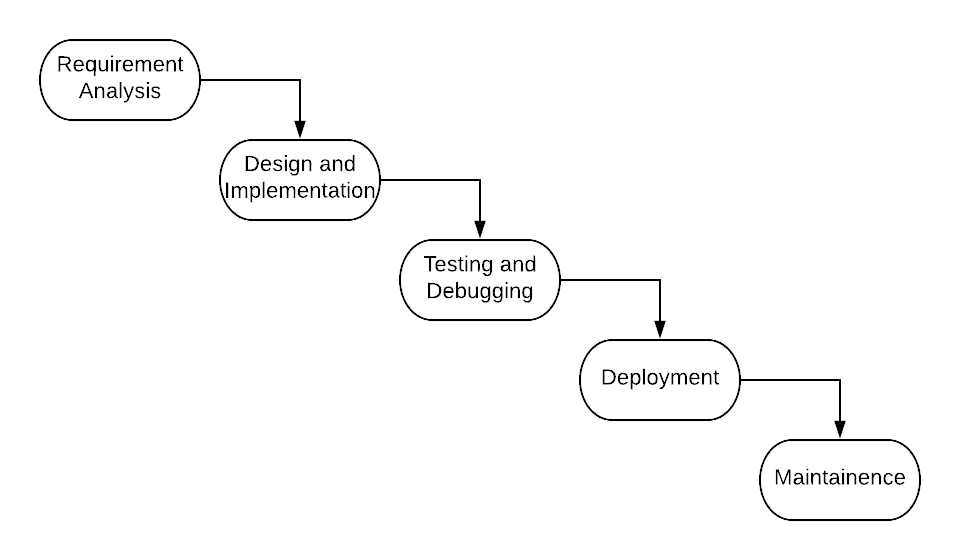
\includegraphics[width=\linewidth]{figures/sdlc.png}
	\centering
	\caption{Proposed software development life cycle}
	\label{fig:sdlc}
\end{figure}

The life cycle begins when the team collects and evaluates the requirements that will be expected from the application. The design and implementation phase will be to design and build both API services and client applications. By the end of this phase, a minimal viable product (MVP) will already have been constructed. In the testing and debugging phases, the quality control methods will be applied to both API and application. Finally, the application will be deployed to Docker containers at the end of the deployment phase. However, there might be slight modifications in the original waterfall model where the design and implementation may be changed slightly after the testing phase if seen as reasonable.

\subsection{Technical Architecture}
The application will be built upon the client-server web architecture, as illustrated in Figure \ref{fig:arch}.

\begin{figure}[H]
    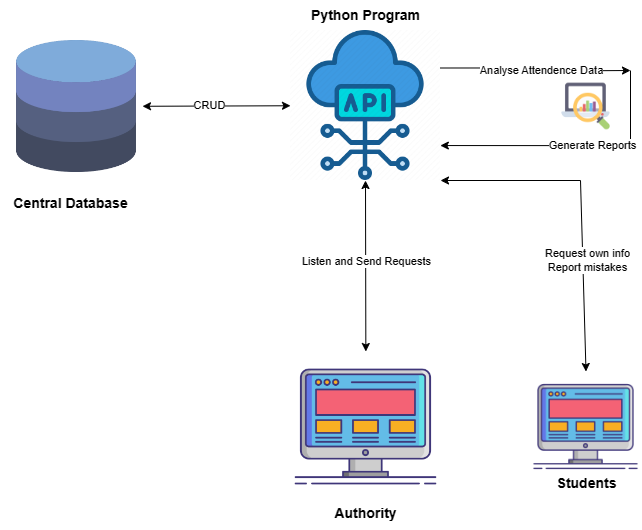
\includegraphics[width=\linewidth]{figures/architecture.png}
    \centering
    \caption{Proposed architecture of the application}
    \label{fig:arch}
\end{figure}

The architecture consists of a database that handles data storage and management. Python is responsible for handling Create, Read, Update, and Delete (CRUD) operations on the database. It also provides WebSocket communication capabilities to the client application.\\

The client application allows students to access their personal attendance information securely. Only authorized personnel, such as administrators or instructors, can access the entire dataset via the client application using WebSocket communication.\\

Python program acts as the intermediary between the client application and is also responsible for generating reports based on the attendance data. This communication ensures seamless integration and efficient report generation.\\

\begin{figure}[H]
    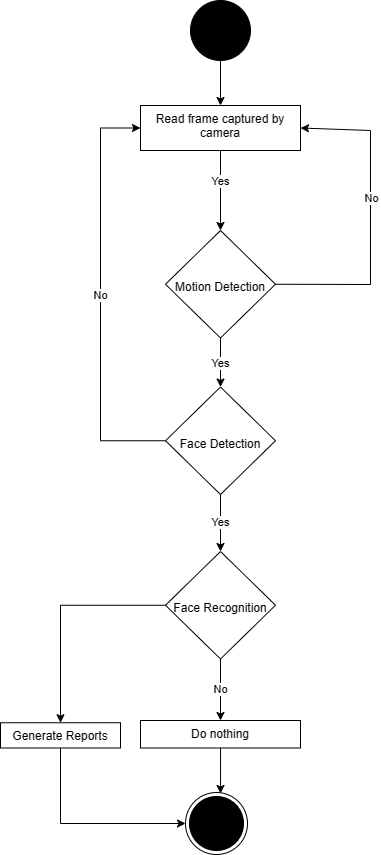
\includegraphics[width=0.6\linewidth]{figures/activity-diagram.png}
    \centering
    \caption{Activity Diagram\cite{yasmeensmart} of the application}
    \label{fig:activity}
\end{figure}

\begin{figure}[H]
    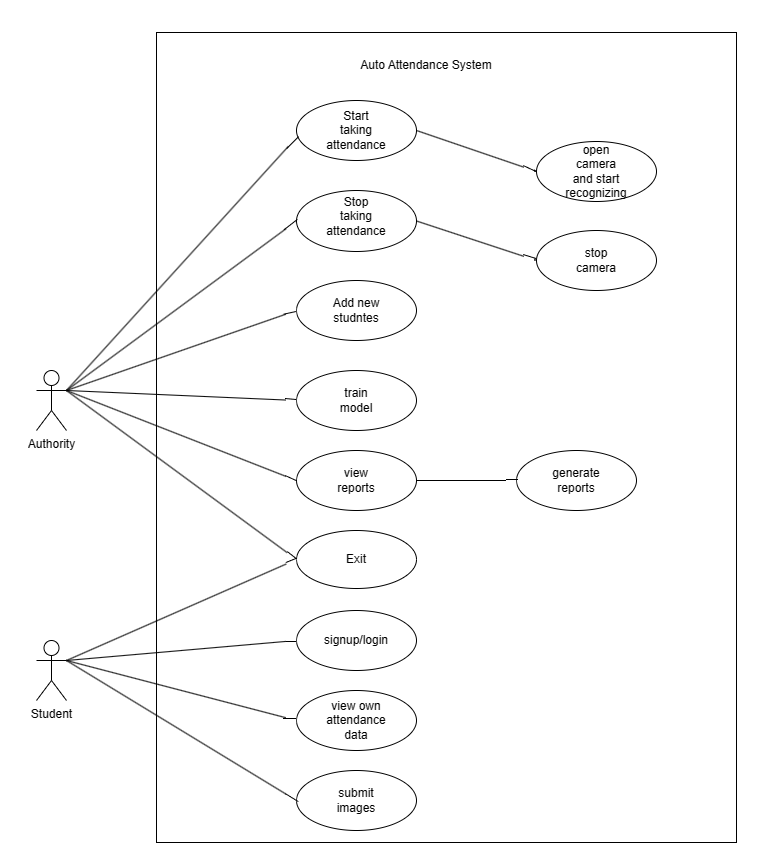
\includegraphics[width=\linewidth]{figures/use-case.png}
    \centering
    \caption{Use-case Diagram of the application}
    \label{fig:usecase}
\end{figure}

\subsection{Proposed Technologies}
Table \ref{table:tech} consists of the major technologies that are proposed to be used during the development and deployment of the application.

\renewcommand{\arraystretch}{1.5}
\begin{table}[H]
\centering
    \begin{tabular}{|l|l|}
        \hline
        \textbf{Subject}    & \textbf{Proposed Technology} \\ \hline
        Backend Database            & PostgreSQL           \\ \hline
        Backend Service    & Python        \\ \hline
        API Communication & WebSocket \\ \hline
        Frontend(Client)  & Next.js(React), Typescript, TailwindCSS              \\ \hline
        Deployment  & Docker Containers              \\ \hline
    \end{tabular}
    \caption{Technologies proposed to be used}
    \label{table:tech}
\end{table}

\subsection{Face detection algorithm}
We plan to utilize the OpenCV library in Python to train the model using students' images and detect faces for attendance purposes. We have two options for face detection: HOG + Linear SVM or MMOD CNN.\\

The HOG + Linear SVM face detector offers faster processing speed compared to the MMOD CNN method. However, it may be less accurate when dealing with changes in the viewing angle or rotation of faces.\\

For more robust face detection, we can employ the MMOD CNN face detector. This approach requires more computational resources, resulting in slower processing times. Nonetheless, it offers higher accuracy and is more resilient to variations in face rotation and viewing angles.\\

Furthermore, if we have access to a GPU, we can leverage it to run the MMOD CNN face detector, enabling real-time face detection. Combining the MMOD CNN face detector with a GPU delivers the perfect combination of deep neural network accuracy and the efficiency of a less computationally demanding model.\\

We have planned to use HOG + Linear SVM because of low resources and less time.\\

The HOG algorithm divides an image into small cells, computes each cell’s gradient orientation and magnitude, and then aggregates the gradient information into a histogram of oriented gradients. These histograms describe the image features and detect objects within an image.

\begin{table}[H]
\centering
\resizebox{\textwidth}{!}{%
\begin{tabular}{|l|l|l|}
\hline
\textbf{Algorithm} & \textbf{HOG + Linear SVM} & \textbf{MMOD CNN} \\
\hline
Approach & Histogram of Oriented Gradients (HOG) feature extraction & Convolutional Neural Network (CNN) \\
\hline
Training Complexity & Less computationally intensive & More computationally intensive \\
\hline
Speed & Faster & Slower \\
\hline
Accuracy & Less accurate, especially with changes in viewing angles & More accurate and robust to face rotation \\
\hline
Face Rotation Tolerance & Low & High \\
\hline
GPU Support & Limited (may not utilize GPU) & Utilizes GPU for improved performance \\
\hline
Model Size & Smaller & Larger \\
\hline
\end{tabular}%
}
\caption{Comparison of HOG + Linear SVM and MMOD CNN algorithms for face detection.}
\label{table:algorithm_comparison}
\end{table}


\newpage

% \section{ Tasks Done so far}
%  We understood the significance of time and aimed to make the most of our development period by maximizing our progress.Within this timeframe, we have made significant progress and successfully completed the following tasks:\\

\begin{itemize}
\item \textbf{Research and Requirements Gathering}: Conducted thorough requirement gathering to ensure alignment with project objectives and user needs.
\item \textbf {Design and User Interface Development}: Successfully designed the system architecture and developed a user-friendly interface including login, sign up, forget password functionality, admin panel, and dashboard.
\item \textbf
{Face Detection and Recognition Technology}: Researched and implemented advanced face detection and recognition technology for accurate attendance tracking.
\item \textbf { Dataset and Model Training}: Made a portal to gather dataset images from students and train the facial recognition model using OpenCV for accurate attendance tracking.
\item\textbf { Database Design and Implementation}: We have successfully designed and implemented the necessary tables, relationships, and entities to store student information, attendance records, and other relevant data while prioritizing efficiency, scalability, and data integrity.
\item\textbf{REST API and websockets}: We connected the backend and frontend using REST APIs for on-demand communication and WebSockets for real-time communication while securing every APIs.
\end{itemize}


By completing these major tasks, we are progressing towards achieving our project goals of developing an automated attendance system that effectively tracks and analyzes student attendance.
% \newpage

% \section{ Performance Analysis and Validation}
% This section focuses on evaluating the effectiveness, efficiency, and reliability of the implemented system. This involves conducting thorough assessments and tests to ensure that the system meets the required performance standards. Here's an overview of the performance analysis and validation aspects:

\begin{itemize}
\item \textbf{Facial Recognition Accuracy:} The accuracy of the facial recognition system is a critical factor in reliable attendance tracking. The performance analysis involves measuring the precision and recall rates of the HOG-based facial recognition method. Through validation, we verify that the system can correctly identify and match students' faces for accurate attendance marking. It struggles a bit when the side view of a student's face is shown. This is mainly due to less number of datasets we are using which is 10 images per student.

\item \textbf{Response Time of APIs and WebSockets}: The speed and responsiveness of the REST APIs and WebSockets are crucial for seamless data transfer and real-time attendance updates. The performance analysis involves measuring the average response time of API requests and WebSocket communication. Validation ensures that the system meets the performance requirements, providing prompt and efficient communication between clients and the server.
Some of the API's response time are as follows
\begin{itemize}
    \item GET: /all-students  20 to 30ms
    \item POST: /create-new-student 300ms
    \item Training time per image 1 to 2s
\end{itemize}
WebSockets are instantaneous once they are connected. 

\item \textbf{System Stability}: The project is made with new and growing technologies like Nextjs and Django, which provides great scalability in the future and is able to handle many concurrent users easily. However, in our case, the number of people accessing the system is very low.

\item \textbf{Authentication Mechanisms}: The authentication mechanisms, including login, login with Google, forgot password, and reset the password, are critical for system security and user access control. The performance analysis involves evaluating the response time and security measures of these authentication processes. Validation ensures that the authentication mechanisms function as intended, providing secure and efficient user authentication.
\end{itemize}

By conducting comprehensive performance analysis and validation, we can identify and address any performance bottlenecks, optimize system components, and ensure that the Presence Project meets the required performance standards. This process helps in delivering a reliable, efficient, and high-performing attendance management solution.
% \newpage

\section{Conclusion}
In conclusion, "Presence: an automated attendance system" represents a much-needed transition from outdated and error-prone manual attendance-tracking methods to a modern, efficient, and web-connected system. The primary goal of this project was to create a facial recognition system for tracking student attendance. Admins provide students with accounts and add their information to the database. The system then detects students' faces using a camera and records their attendance in the database. Both teachers and admins have access to attendance reports.\\

Throughout this project, we conducted extensive research on various face recognition algorithms and selected the most suitable one, which happens to be HOG. We employed diverse techniques and programming languages to develop the system, thoroughly tested it, and achieved success. As a result, this system can now be implemented to efficiently manage student attendance records.\\

Looking ahead, there is ample potential for further development. Additional features beneficial to both students and teachers, such as assignment tracking, result recording, and grade management, could be seamlessly integrated into the system.

\newpage


 \section{Further Works / Recommendations }
\begin{itemize}
\item \textbf {Record attendance for each subject}: For now we are only recording attendance for a day. In future We will add functionality to record the attendance of each subject for better reports and insights.

\item \textbf { Enhance Facial Recognition Accuracy}: improving the facial recognition algorithms to ensure high accuracy, especially in challenging conditions, such as low light or varying student appearances (e.g., facial hair, makeup, or accessories).

\item \textbf{ Mobile Integration}: Develop a mobile app for students to easily track their attendance using their smartphones, providing an additional convenience layer to the system.

\item \textbf{ Customization Options}: Provide customization features that allow educational institutions to tailor the system to their specific needs, including attendance policies and reporting formats.


\end{itemize}



\newpage

% \section{Tasks Remaining }
% With a significant portion of our project already completed, there are still several important tasks remaining to be accomplished. These tasks will require our focused attention and effort to ensure the successful delivery of our automated attendance system. The following are the tasks that are yet to be completed:

\begin{itemize}
\item \textbf {Record attendance for each subject}: For now we are only recording attendance for a day. We are planning to add functionality to record the attendance of each subject for better reports and insights.

\item \textbf { Data Analysis and Report Generation}: Analyze the collected attendance data to derive insights and generate comprehensive reports for educators and administrators.

\item \textbf{ Testing and Validation}: Conduct user testing to ensure system functionality, perform integration testing, evaluate performance, and validate the accuracy of attendance tracking.

\item \textbf{ User Testing}: Engage users to obtain feedback on usability and implement improvements based on their suggestions.

\item \textbf{ Deployment }: Make ready-to-use deployment containers with Docker for backend services and host the frontend application to Vercel.  

\end{itemize}

With the remaining time in the project timeline, we will focus on implementing the remaining functionalities, conducting thorough testing and quality assurance, and refining the system based on user feedback. Our objective is to deliver a fully functional and reliable automated attendance system that meets the expectations and requirements of our users.


% \newpage

% \section{Deliverable/Output}
% The proposed deliverables for the Presence project align with the defined architecture and project objectives. These deliverables encompass various components and functionalities of the automated attendance system, ensuring a comprehensive solution for tracking and analyzing student attendance.\\

\textbf{Database Design and Implementation}\\
The first deliverable involves designing and implementing the database architecture that will serve as the backbone of the Presence system. This includes creating the necessary tables, relationships, and entities to store student information, attendance records, subject details, and other relevant data. The database design will prioritize efficiency, scalability, and data integrity.\\

\textbf{NodeJS Application}\\
The NodeJS application will form a crucial component of the Presence system. It will handle the communication between the database and the client application, enabling CRUD operations and WebSocket communication. The deliverable will include the development and deployment of the NodeJS application, ensuring its stability, security, and seamless integration with other system components.\\

\textbf{Client Application}\\
The client application will provide a user-friendly interface for students to access their attendance information securely. It will be designed with intuitive navigation, responsive design, and robust authentication mechanisms. The deliverable will include the development of the client application, ensuring compatibility across different devices and browsers.\\

\textbf{FaceML Access and Reporting}\\
The Presence system will offer authorized personnel, such as administrators or instructors, access to comprehensive attendance data and reporting functionalities. This deliverable involves developing a secure login system for authorities, granting them access to view and analyze attendance records, generate reports, and gain insights into attendance patterns and subject preferences. The reporting component will leverage Python programs to generate insightful reports based on the collected data.
% \newpage

\section{Project Task and Time schedule}

The working time period for the project was four months. The project was completed by the end of the spring semester as per the requirements of the university. The major task division among the team members was mentioned in the table. \ref{table:taskdiv}.

\begin{table}[H]
\centering
\begin{tabular}{|l|l|}
\hline
\textbf{Team Member} & \textbf{Assigned Task}                                   \\ \hline
Rupesh Budhathoki    & Project Management, Overall Coordination, FullStack Development \\ \hline
Apsara Bishwokarma   & Frontend Development                     \\ \hline
Sampada Kharel       & Backend Development            \\ \hline
Sudarshan Kshettry   & FullStack Development\\ \hline
\end{tabular}
\caption{Division of tasks among project team members}
\label{table:taskdiv}
\end{table}

The time schedule for the development of the project was illustrated in the following Gantt chart.\\

\begin{table}[ht]
  \centering
    \begin{ganttchart}[
        vgrid={*{4}{draw=none}, dotted},
        hgrid,
        x unit=0.7cm,
        y unit chart=0.8cm,
        bar/.append style={fill=cyan!60, rounded corners=2pt},
        bar incomplete/.append style={fill=yellow!60},
        title/.append style={draw=none, fill=white},
        title label font=\bfseries\small,
        bar label font=\small,
        milestone label font=\small,
        group label font=\small\bfseries,
    ]{1}{16}
        \gantttitle{Weeks}{16} \\
        \gantttitlelist{1,...,16}{1} \\
        \ganttgroup{Project Phases}{1}{16} \\
        \ganttbar{Requirement Analysis}{1}{2} \\
        \ganttbar{Design and Implementation}{3}{12} \\
        \ganttbar{Testing and Debugging}{11}{14} \\
        \ganttbar{Deployment}{14}{15} \\
        \ganttmilestone{Maintenance}{16} \\
    \end{ganttchart}
  \caption{Gantt Chart}
\end{table}
\newpage

\newpage
\section{References}
\printbibliography[heading=none]


\section{Appendix}
To ensure the security and accessibility of the system, we have implemented various authentication mechanisms, including:
\begin{itemize} 
\item \textbf{Login}: Users can securely login using their credentials to access the system's features and functionalities.
\begin{figure}[H]
    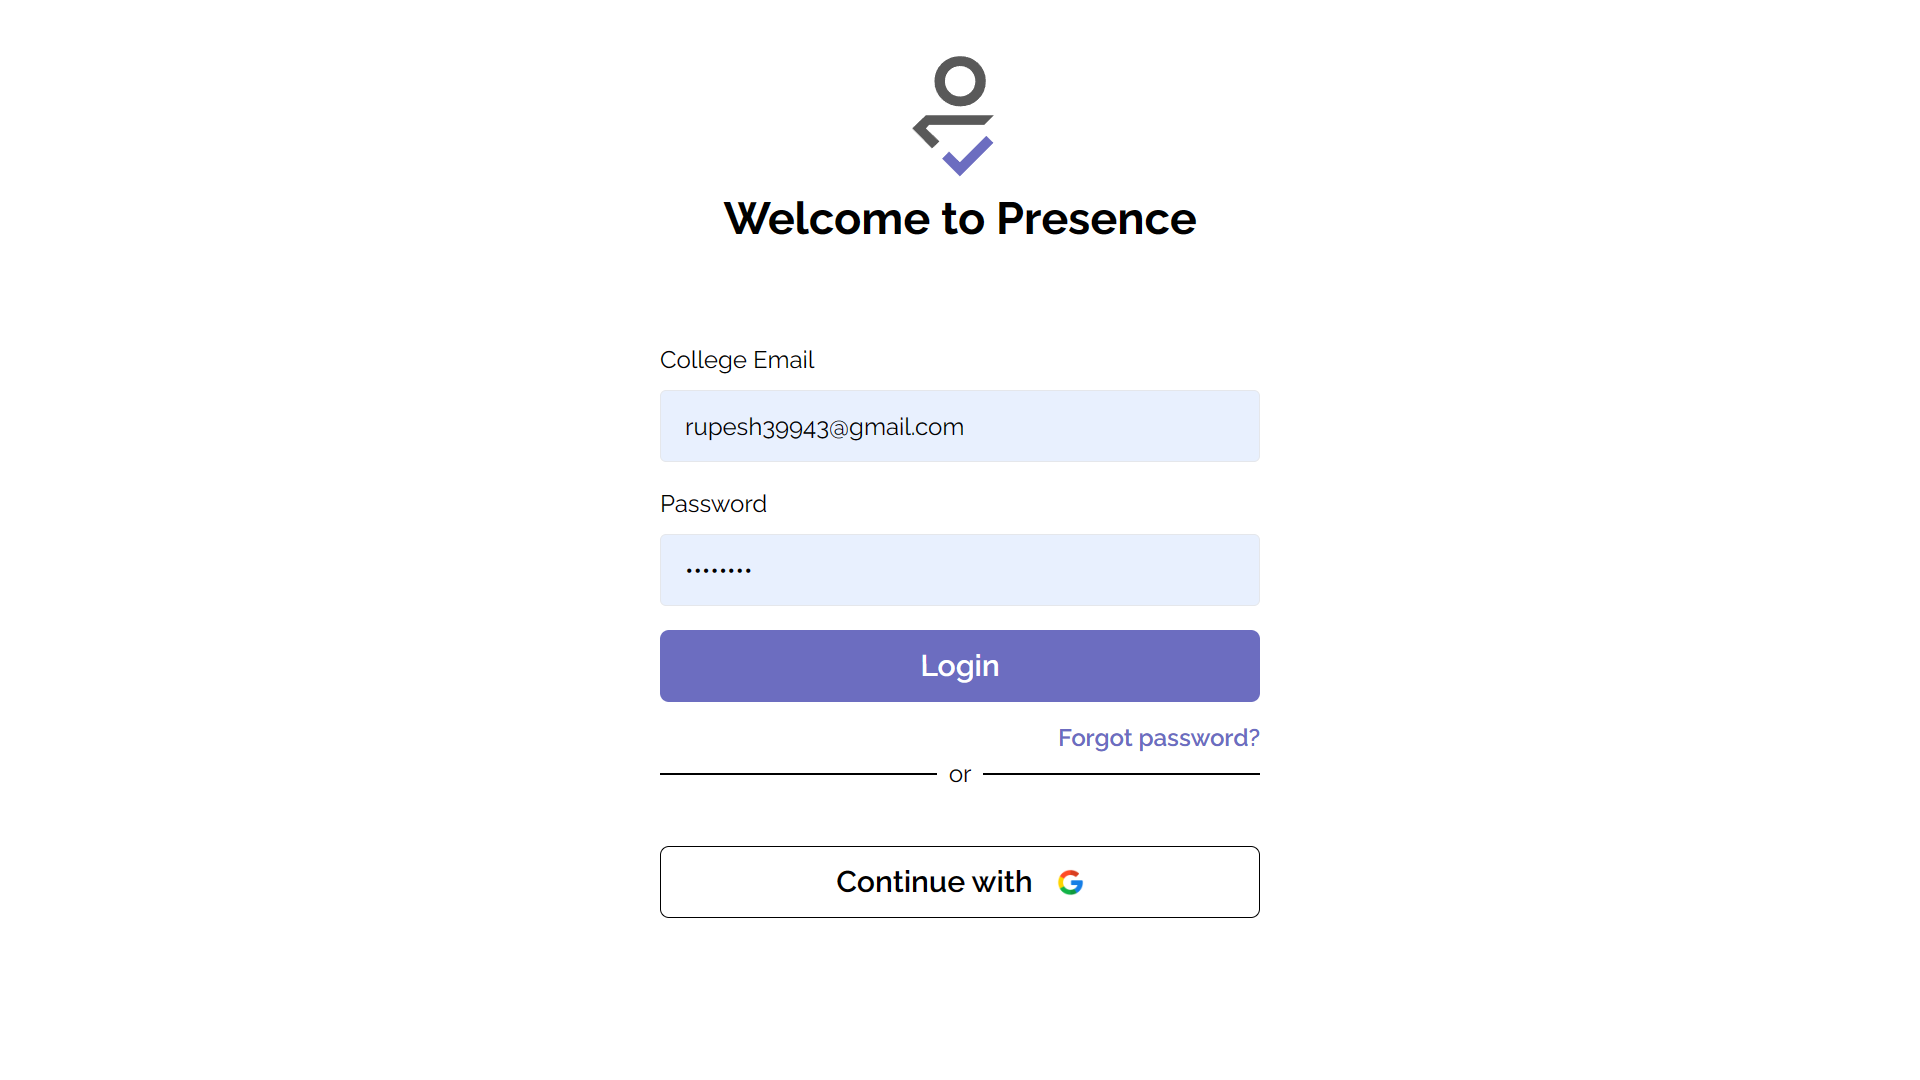
\includegraphics[width=\linewidth]{figures/login.png}
    \centering
    \caption{Login form for both users and admin}
\end{figure}
\item \textbf{Login with Google}: Users have the option to authenticate themselves using their Google accounts, providing a convenient and streamlined login experience.
\begin{figure}[H]
    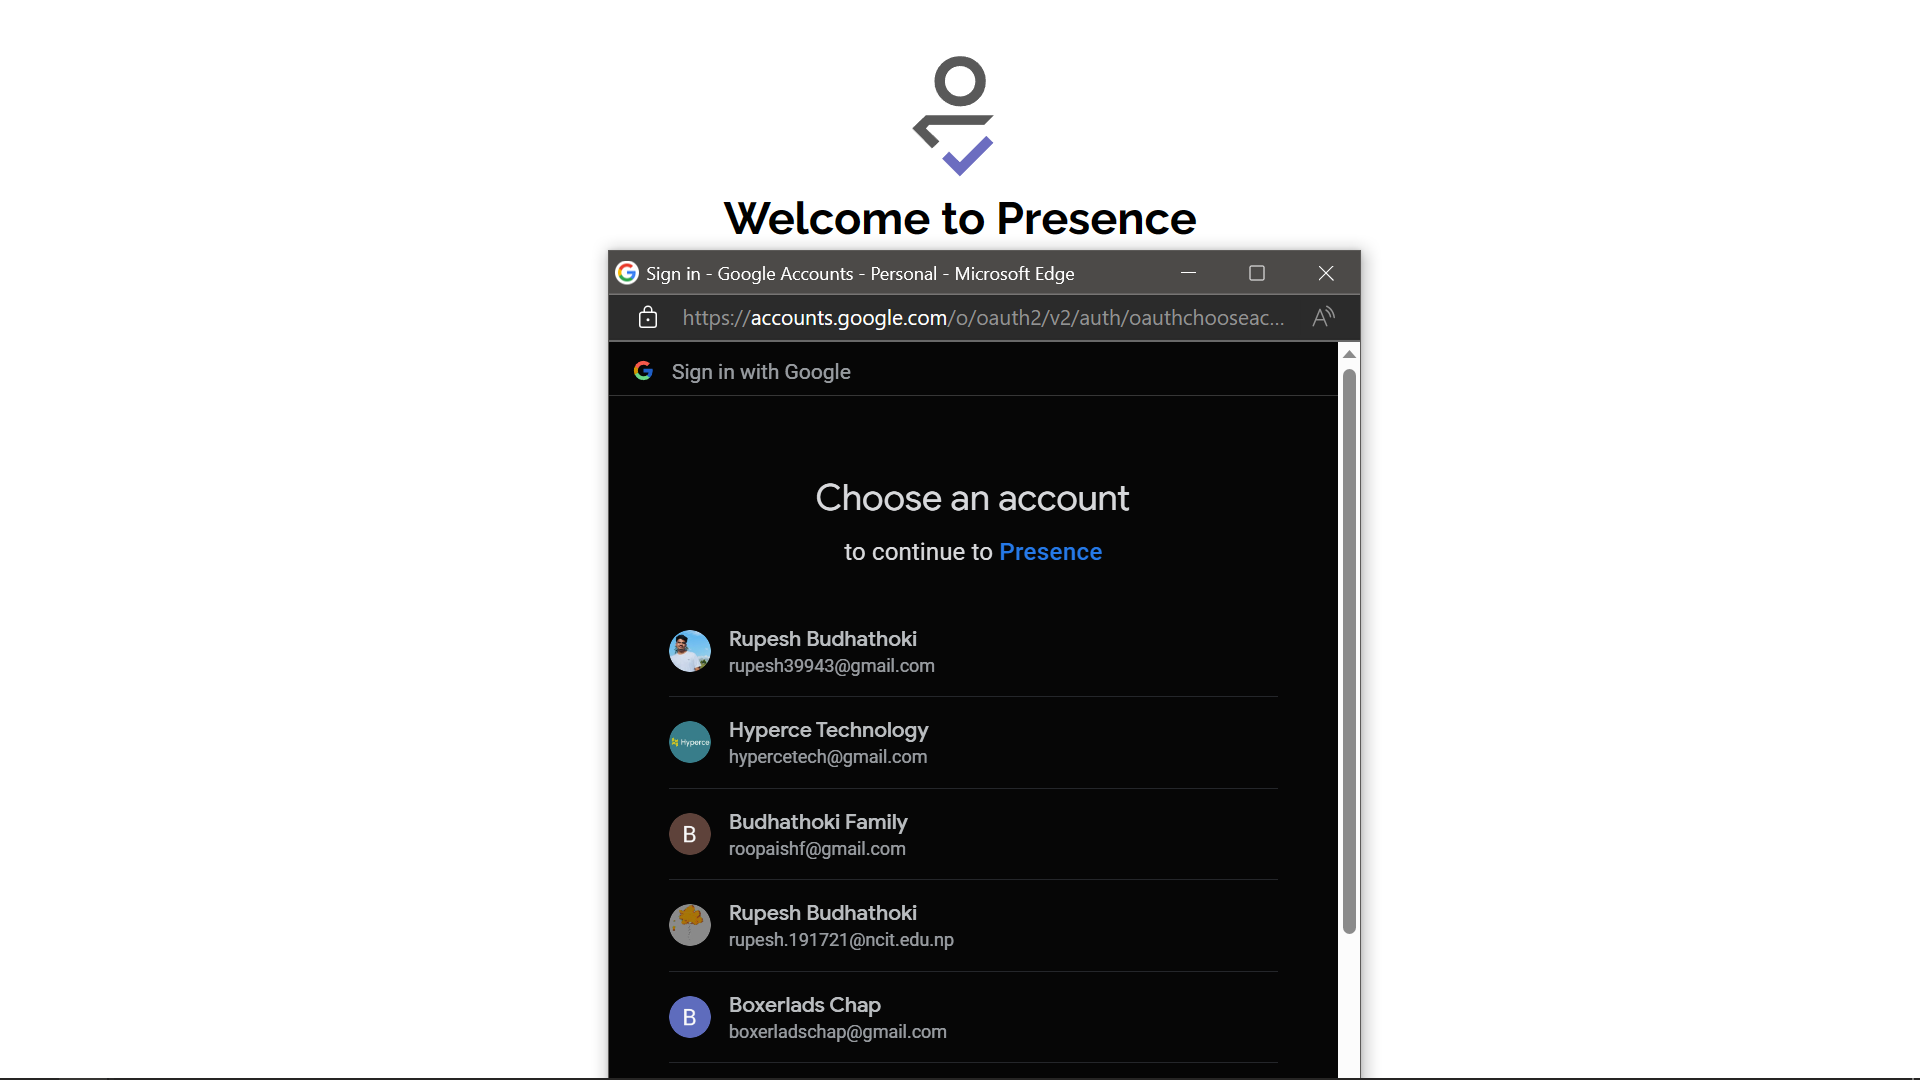
\includegraphics[width=\linewidth]{figures/login-with-google.png}
    \centering
    \caption{Login with Google functionality}
\end{figure}
\item \textbf{Forgot Password}: In the event of a forgotten password, a password recovery mechanism allows users to reset their passwords securely.
\begin{figure}[H]
    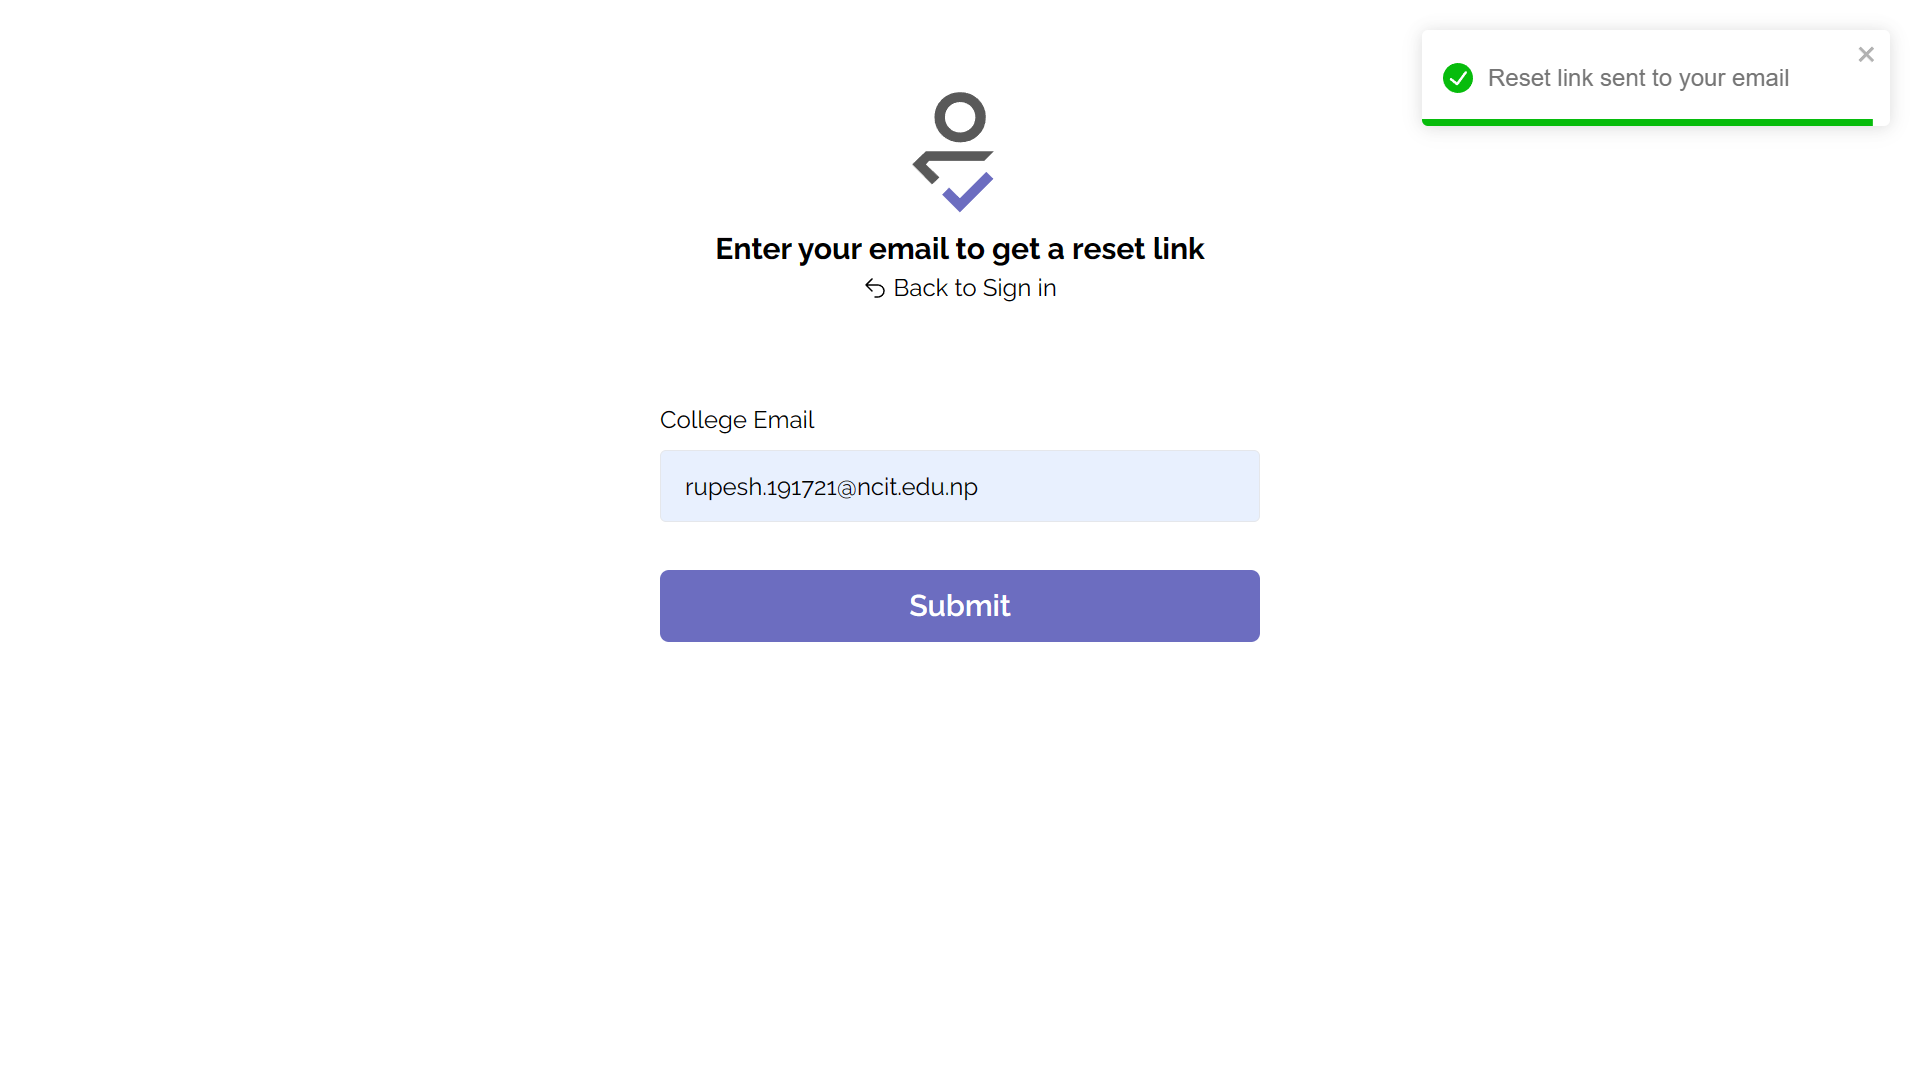
\includegraphics[width=\linewidth]{figures/forgot-password.png}
    \centering
    \caption{Login with google functionality}
\end{figure}
\item \textbf{Reset Password}: Users can initiate the password reset process and set a new password to regain access to their accounts.
\begin{figure}[H]
    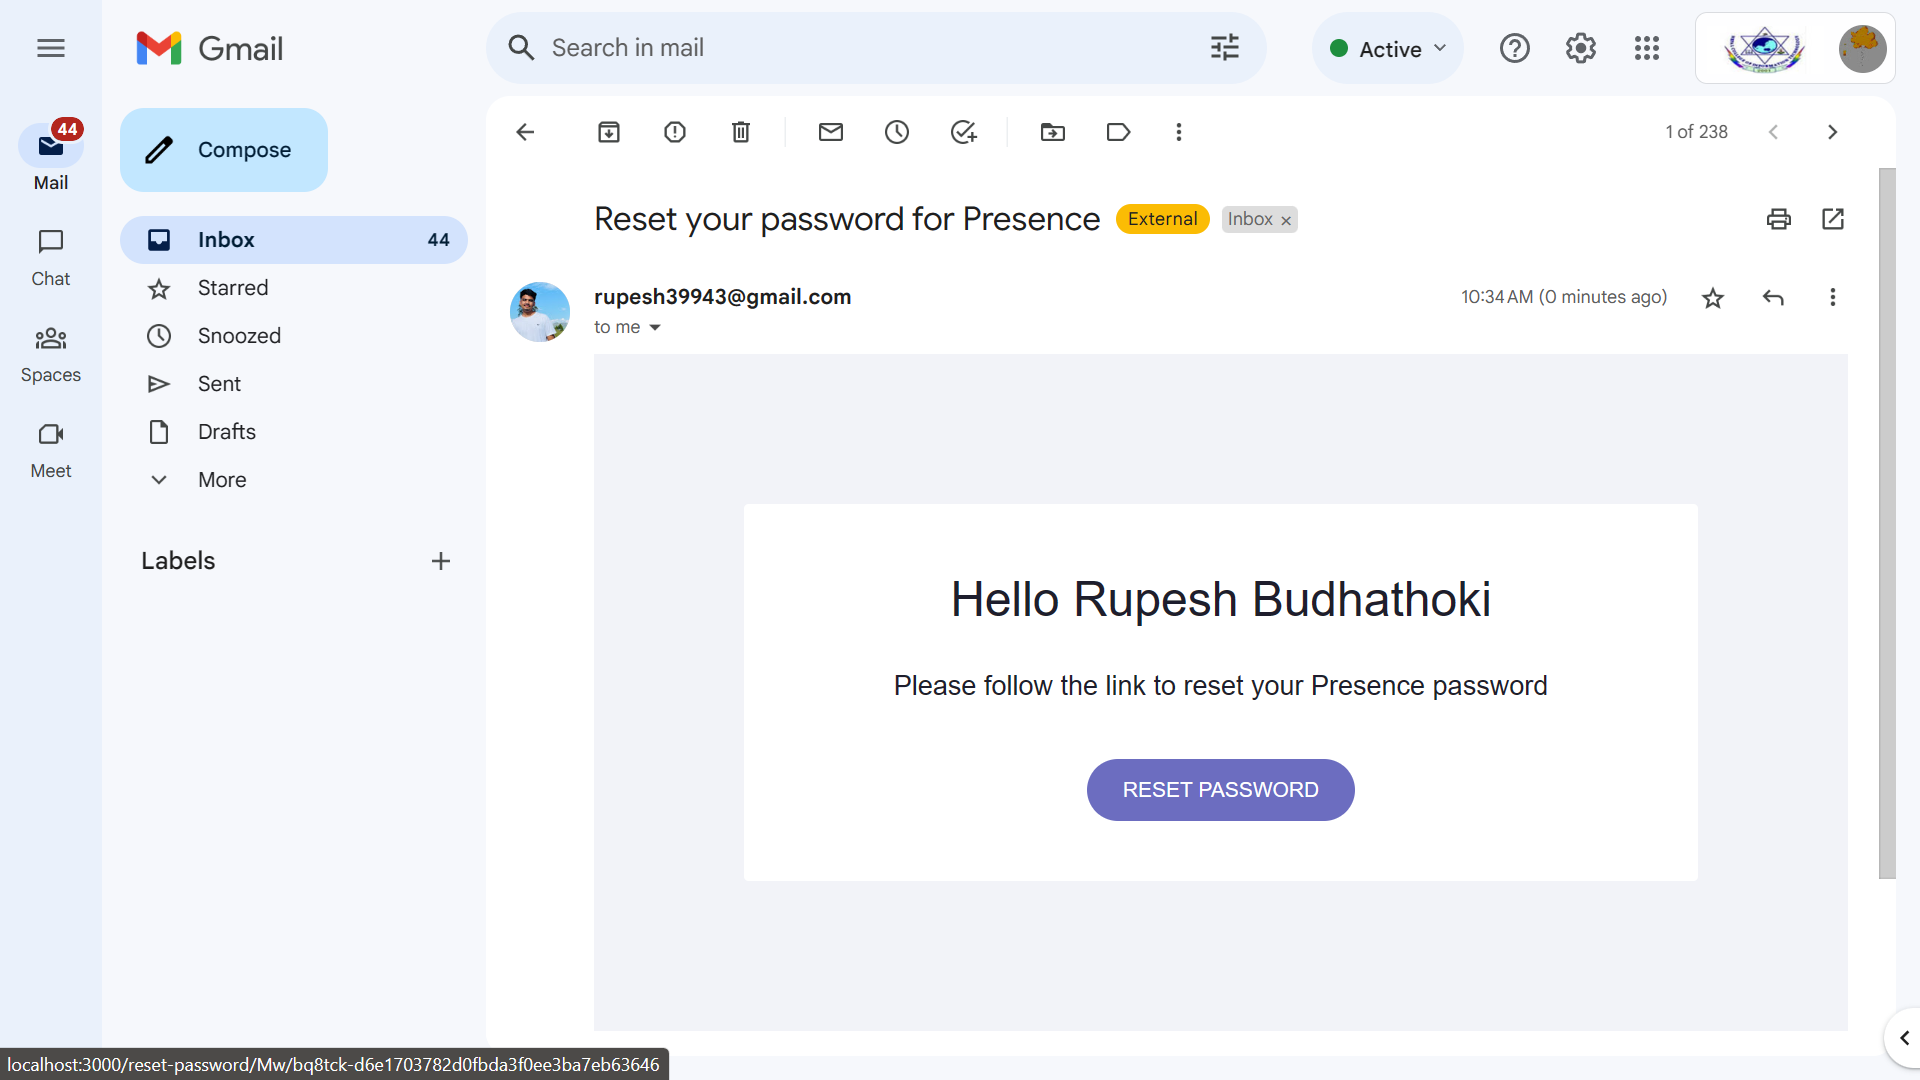
\includegraphics[width=\linewidth]{figures/reset-pw-email.png}
    \centering
    \caption{Reset Password Email}
\end{figure}
\begin{figure}[H]
    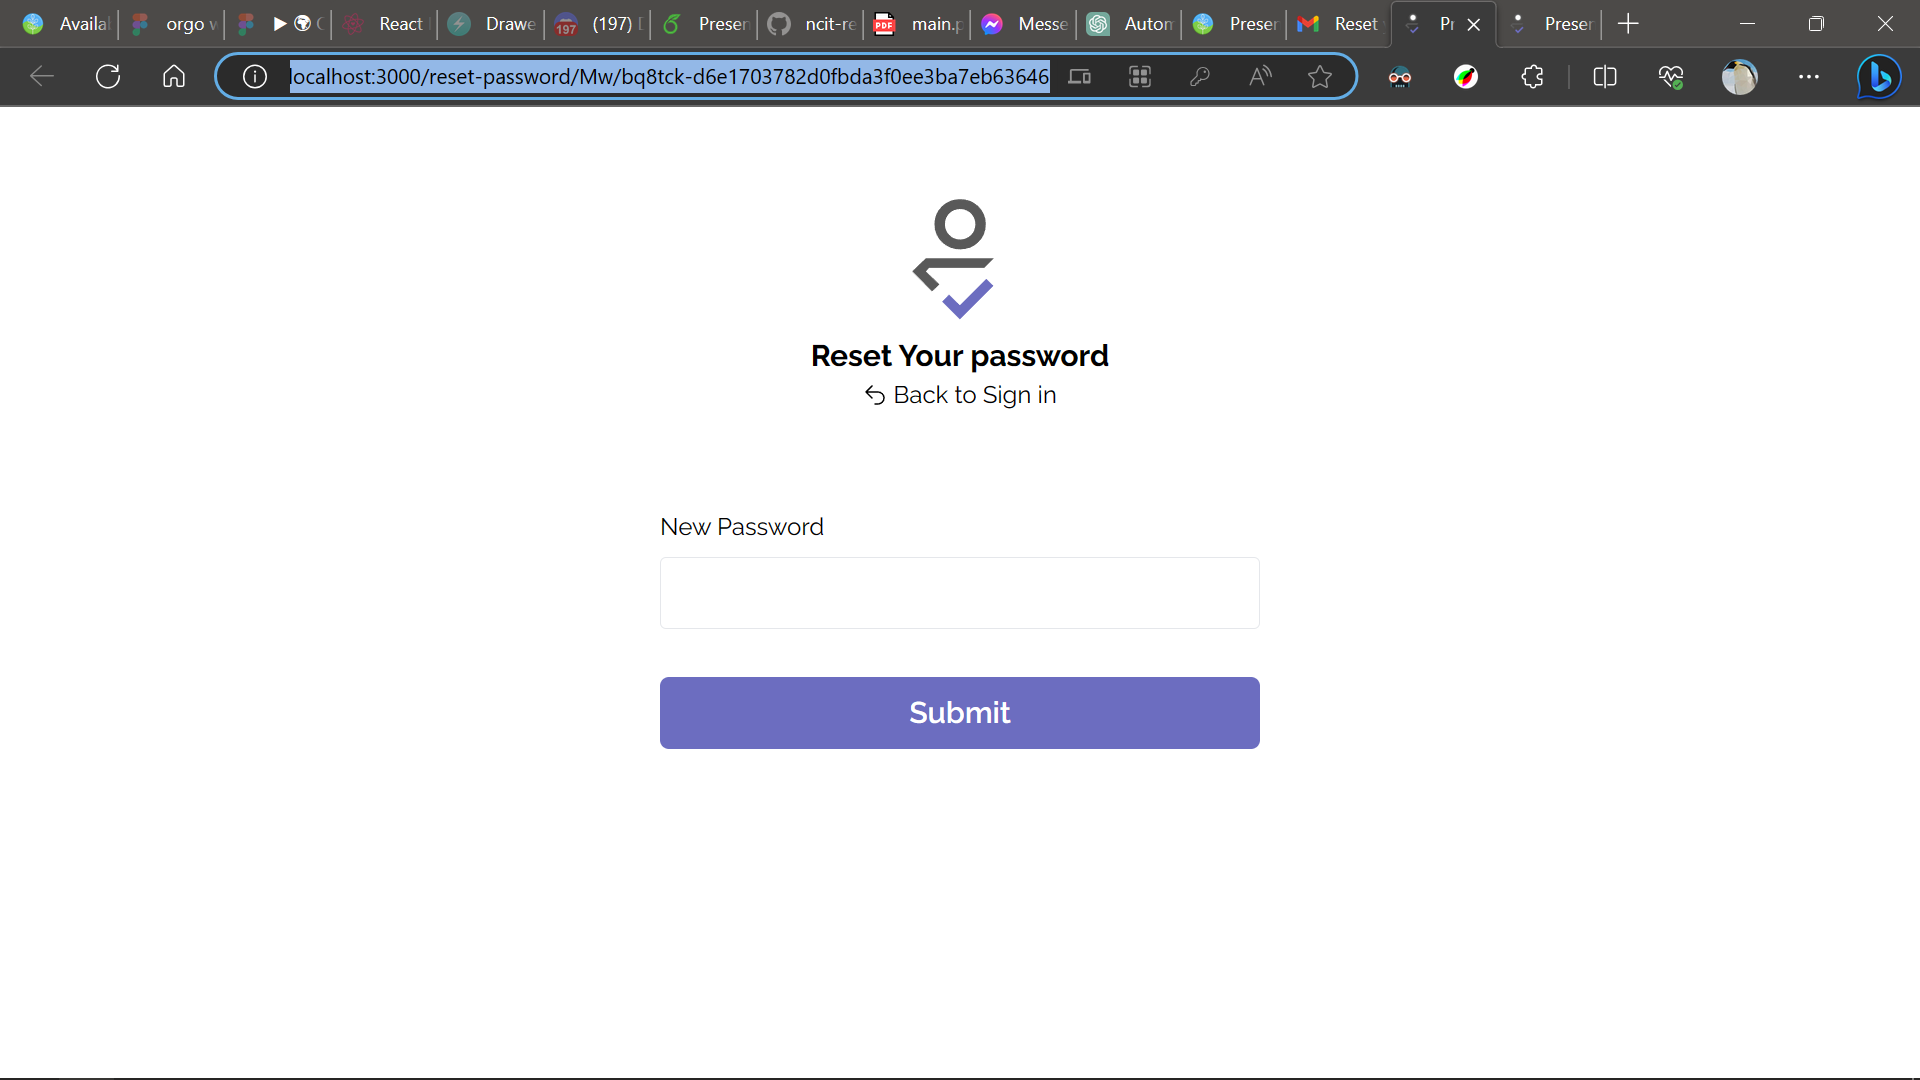
\includegraphics[width=\linewidth]{figures/reset-pw.png}
    \centering
    \caption{Reset password}
\end{figure}
\end{itemize}

Key Features for Students:
\begin{itemize} 
\item \textbf{Image Submission}: Students can submit their images to be used for facial recognition and attendance tracking.
\begin{figure}[H]
    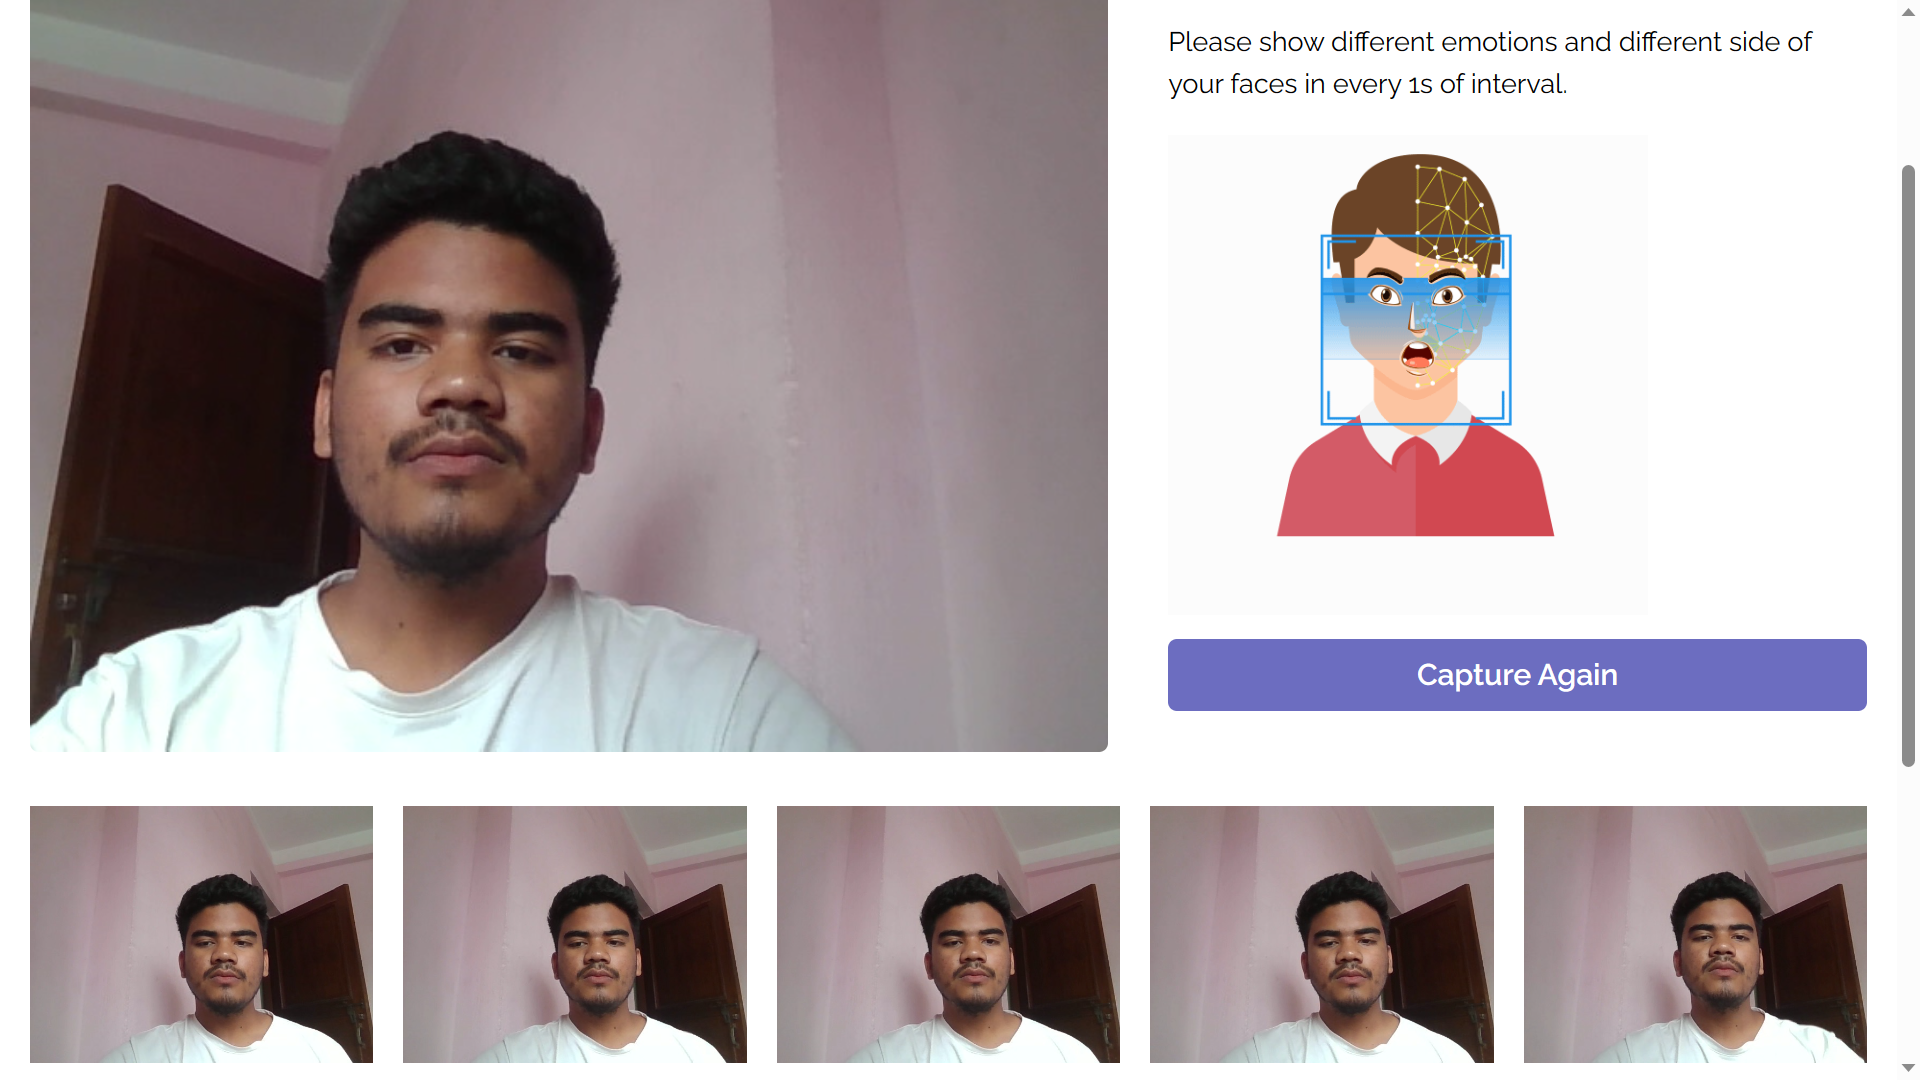
\includegraphics[width=\linewidth]{figures/submit-images.png}
    \centering
    \caption{Image submission form}
\end{figure}
\item \textbf{Attendance Tracking}: Students have access to view their attendance records, providing insights into their attendance patterns and history.
\begin{figure}[H]
    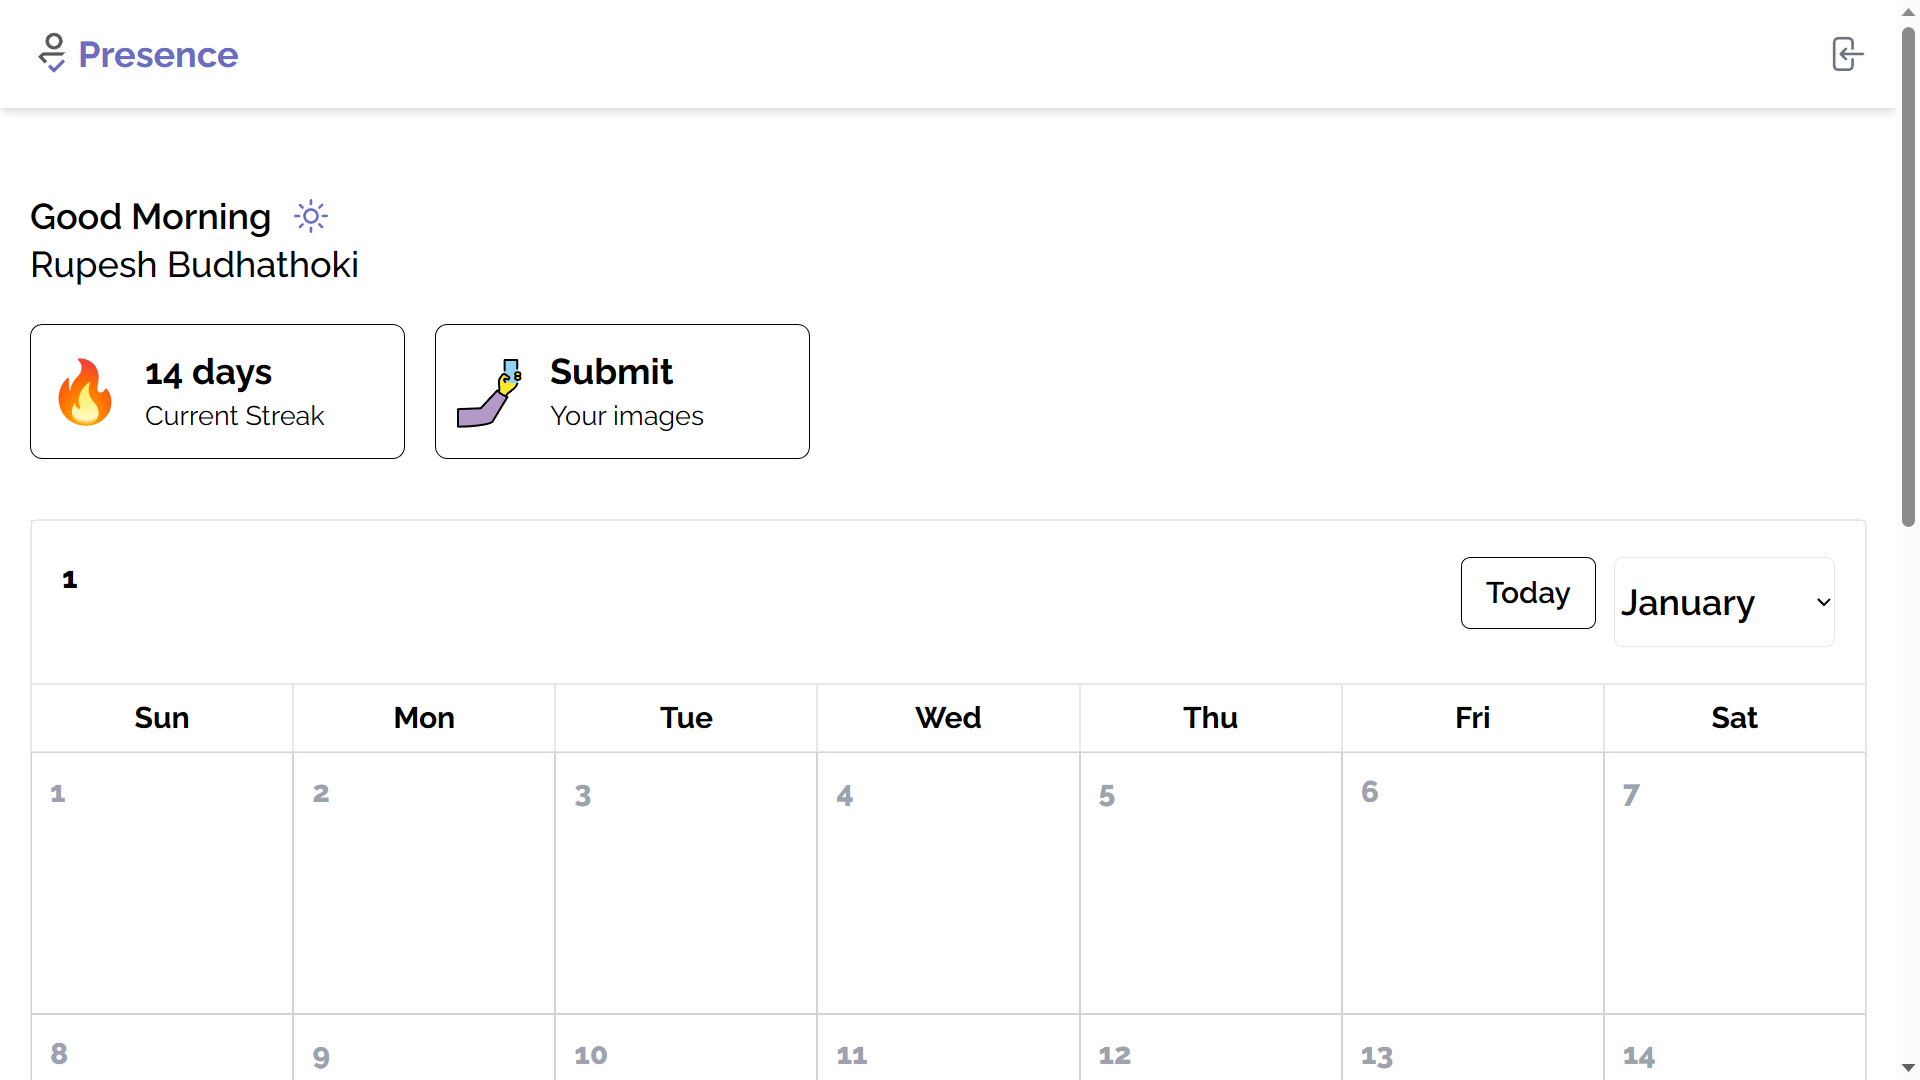
\includegraphics[width=\linewidth]{figures/student-dash.png}
    \centering
    \caption{Student dashboard}
\end{figure}
\end{itemize}


Key Features for Authorities:
\begin{itemize} 
\item \textbf{Student Management}: Authorities can add new students to the system, maintaining an up-to-date database of enrolled individuals.
\begin{figure}[H]
    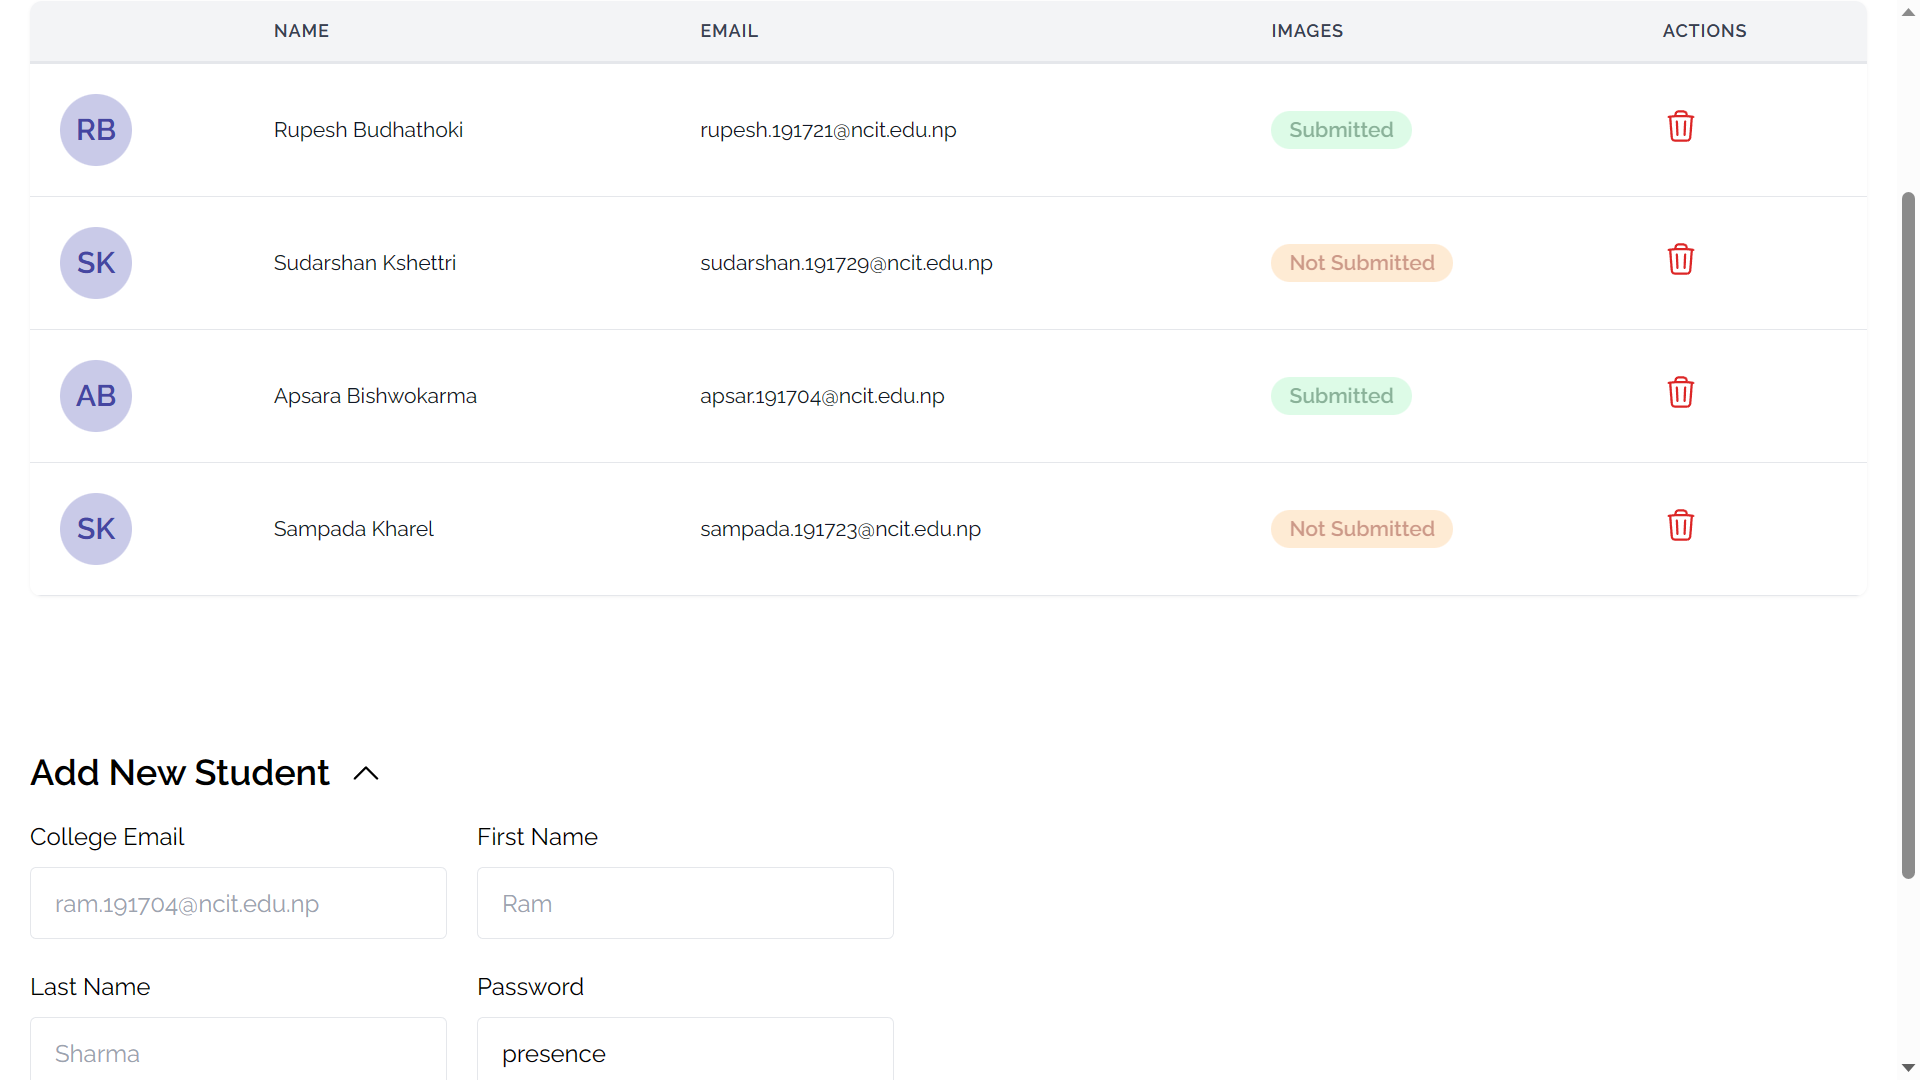
\includegraphics[width=\linewidth]{figures/students-list.png}
    \centering
    \caption{Student Management}
\end{figure}
\item \textbf{Model Training}: Authorities have the ability to train the facial recognition model using images submitted by students, ensuring accurate and reliable attendance detection.
\begin{figure}[H]
    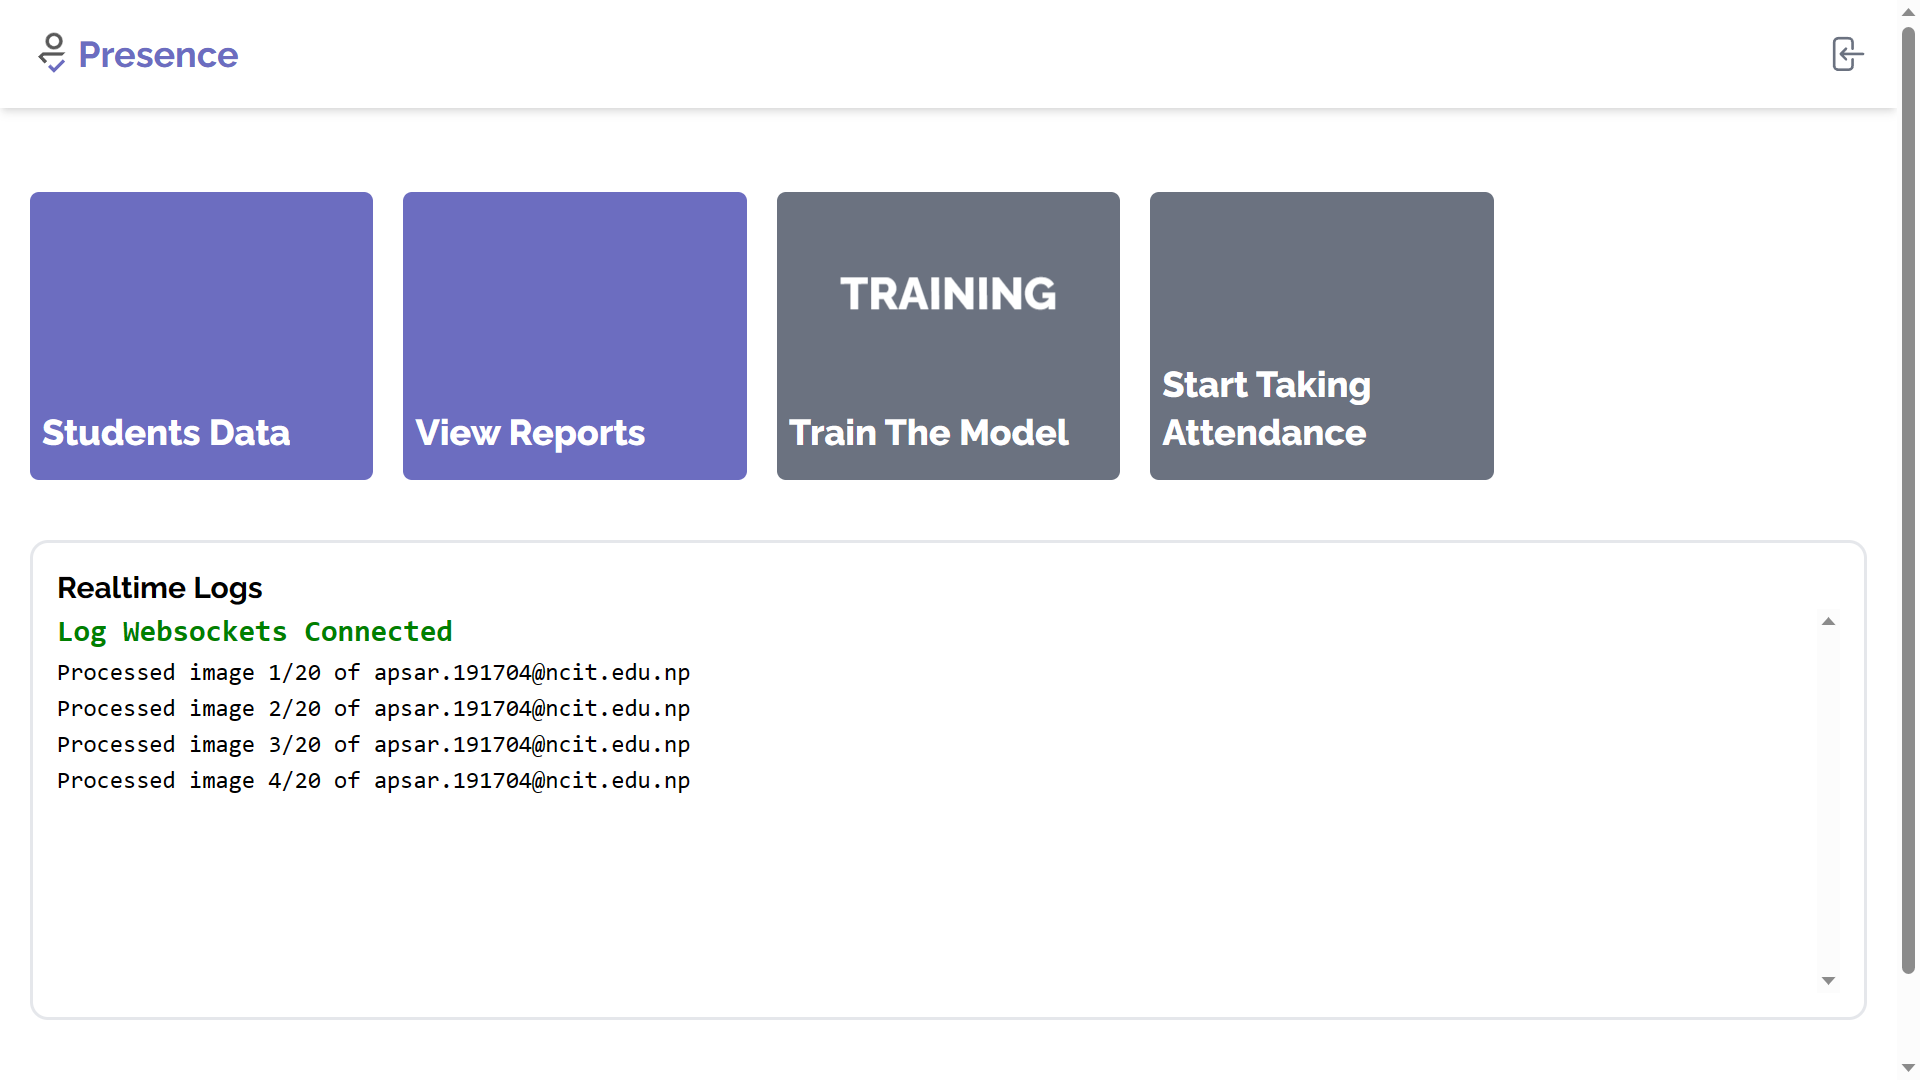
\includegraphics[width=\linewidth]{figures/training.png}
    \centering
    \caption{Training model with images submitted by students}
\end{figure}
\item \textbf{Real-time Attendance}: Authorities can initiate the real-time attendance process, enabling the system to mark attendance as students are recognized.
\begin{figure}[H]
    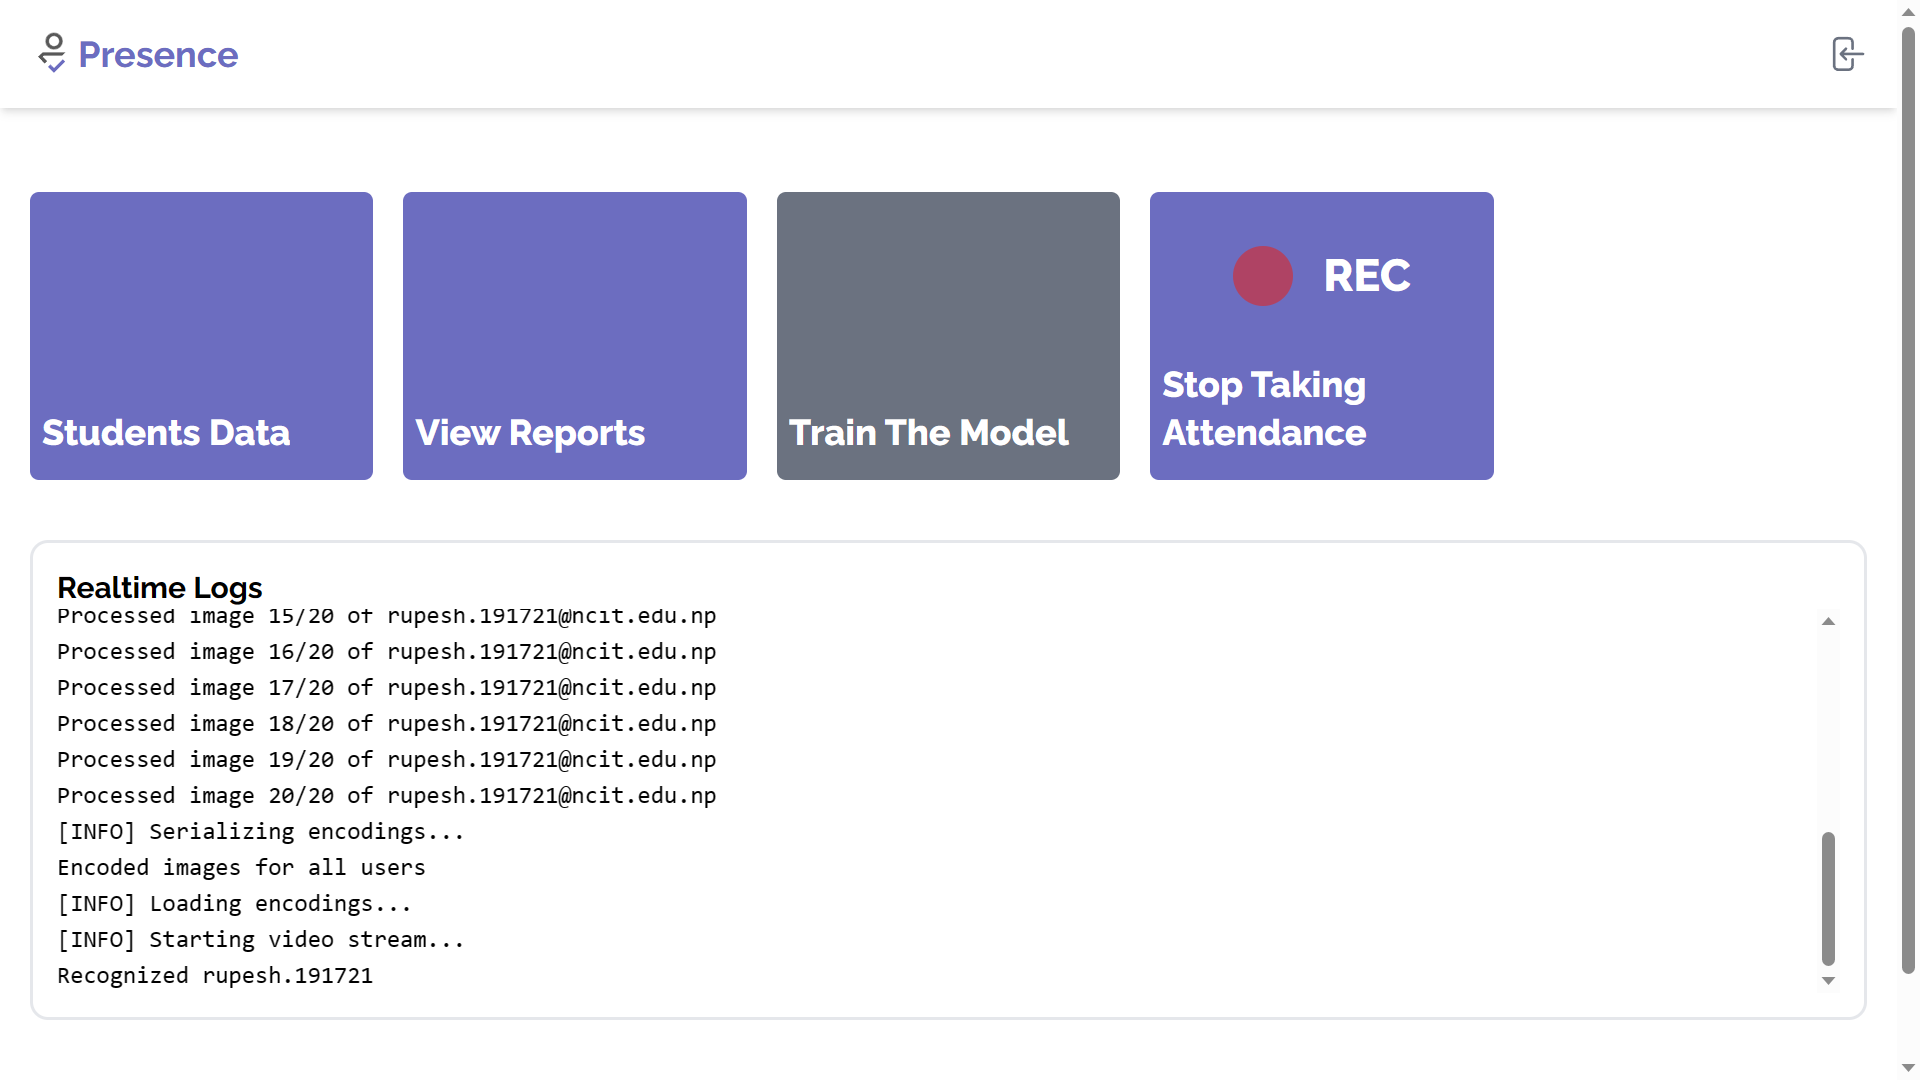
\includegraphics[width=\linewidth]{figures/taking-attendance.png}
    \centering
    \caption{Realtime attendance log}
\end{figure}
\begin{figure}[H]
    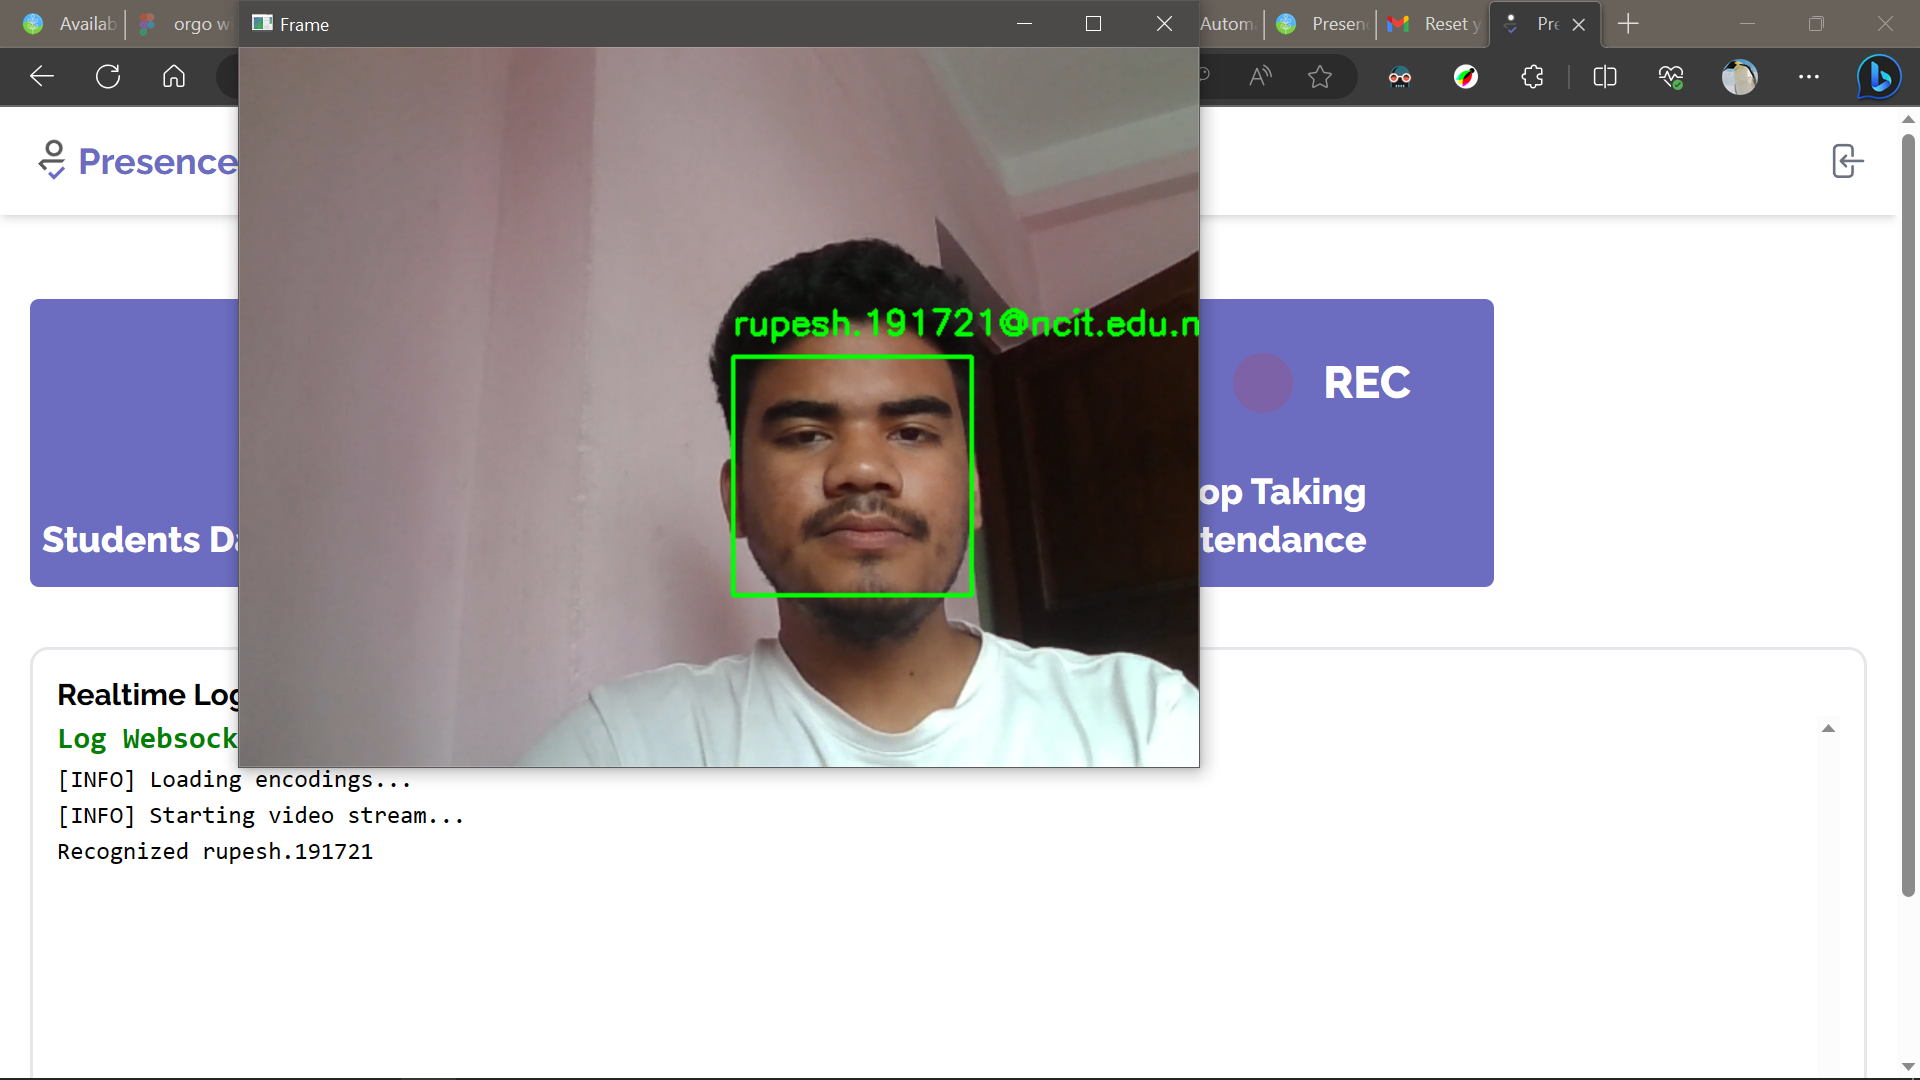
\includegraphics[width=\linewidth]{figures/python-cam.png}
    \centering
    \caption{Realtime attendance from cam}
\end{figure}

\item \textbf{Student Calendar}: Student attendance status.
\begin{figure}[H]
    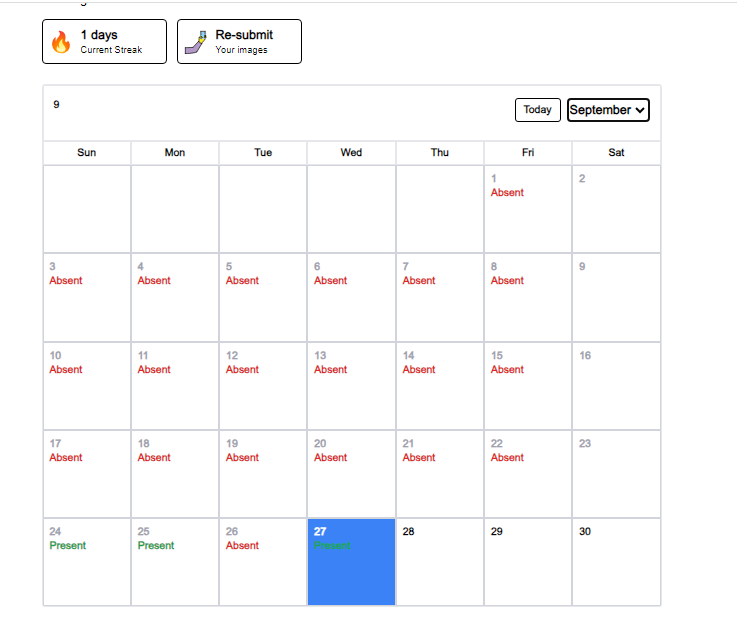
\includegraphics[width=\linewidth]{figures/student-calendar.png}
    \centering
    \caption{Student Calendar}
\end{figure}

\item \textbf{Encode Faces}: Code snippet to encode faces and make a pickle file.

\begin{minted}{python}

@user_passes_test(lambda u: u.is_superuser)
def encode_images(request):
    dataset_path = 'datasets'
    encodings_path = 'encodings.pickle'
    channel_layer = get_channel_layer()

    async_to_sync(channel_layer.group_send)(
        'status_group',
        {
            'type': 'status_message',
            'message': "encoding_images"
        }
    )

    if not os.path.exists(dataset_path):
        return JsonResponse({'success': False, 'message':
        'Dataset directory not found'}, status=400)

    image_paths = list(paths.list_images(dataset_path))

    known_encodings = []
    known_names = []

    for (i, image_path) in enumerate(image_paths):
        name = os.path.basename(os.path.dirname(image_path))
        image = cv2.imread(image_path)
        rgb = cv2.cvtColor(image, cv2.COLOR_BGR2RGB)

        boxes = face_recognition.face_locations(rgb)
        encodings = face_recognition.face_encodings(rgb, boxes)

        for encoding in encodings:
            known_encodings.append(encoding)
            known_names.append(name)

        async_to_sync(channel_layer.group_send)(
            'log_group',
            {
                'type': 'log_message',
                'message': f"""Processed image
                {i+1}/{len(image_paths)} of {name}"""
            }
        )

    async_to_sync(channel_layer.group_send)(
        'log_group',
        {
            'type': 'log_message',
            'message': f"[INFO] Serializing encodings..."
        }
    )
    data = {"encodings": known_encodings, "names": known_names}
    with open(encodings_path, "wb") as f:
        f.write(pickle.dumps(data))

    async_to_sync(channel_layer.group_send)(
        'log_group',
        {
            'type': 'log_message',
            'message': "Encoded images for all users"
        }
    )
    async_to_sync(channel_layer.group_send)(
        'status_group',
        {
            'type': 'status_message',
            'message': "none"
        }
    )

    return JsonResponse({'success': True})


stop_stream = False
\end{minted}

\item \textbf{Take Attendance}: Code snippet to take attendance of users.

\begin{minted}{python}

@user_passes_test(lambda u: u.is_superuser)
@csrf_exempt
def take_attendance(request):
    global stop_stream


    if request.method == 'POST':
        json_data = json.loads(request.body)
        display_video = json_data.get('display_video') or False
        model = json_data.get('model') or 'hog'
        day = date.today().day
        month = date.today().month
        year = date.today().year
        
    # return JsonResponse({'success': month, 'message': 'month'},status=200)
         

        if Attendance.objects.filter(day=day, month=month, year=year).exists():
            return JsonResponse({'success': day, 'message': """Attendance 
            for today is already taken"""}, status=200)

        channel_layer = get_channel_layer()
        dataset_path = 'datasets'
        encodings_path = 'encodings.pickle'
        image_paths = list(paths.list_images(dataset_path))

        if not os.path.exists(dataset_path):
            return JsonResponse({'success': False, 'message': """Dataset 
            directory not found"""}, status=400)

        # Load the known faces and embeddings
        async_to_sync(channel_layer.group_send)(
            'log_group',
            {
                'type': 'log_message',
                'message': "[INFO] Loading encodings..."
            }
        )
        async_to_sync(channel_layer.group_send)(
            'status_group',
            {
                'type': 'status_message',
                'message': "taking_attendance"
            }
        )
        data = pickle.loads(open(encodings_path, "rb").read())
        # Initialize the video stream and allow the camera sensor
        # to warm up
        async_to_sync(channel_layer.group_send)(
            'log_group',
            {
                'type': 'log_message',
                'message': "[INFO] Starting video stream..."
            }
        )
        vs = VideoStream(src=0).start()
        time.sleep(2.0)

        detected_users = []
        names = []
        # get all users and make a list of {name, email}
        attendance_stream = {
            'present_users': [],
            'absent_users': [],
        }
        users = User.objects.all()
        for user in users:
            attendance_stream['absent_users'].append({
                'name': user.first_name + ' ' + user.last_name,
                'email': user.email
            })

        today = date.today()
        attendance_queryset = Attendance.objects.filter(
            day=today.day, month=today.month, year=today.year)

        # Loop over frames from the video file stream
        while True:
            if stop_stream:
                break
            # Grab the frame from the threaded video stream
            frame = vs.read()

            # Convert the input frame from BGR to RGB 
            # then resize it to have
            # a width of 750px (to speed up processing)
            rgb = cv2.cvtColor(frame, cv2.COLOR_BGR2RGB)
            rgb = imutils.resize(frame, width=750)
            r = frame.shape[1] / float(rgb.shape[1])
            # Detect the (x, y)-coordinates of the bounding boxes
            # corresponding to each face in the input frame, then compute
            # the facial embeddings for each face
            boxes = face_recognition.face_locations(rgb, model=model)
            encodings = face_recognition.face_encodings(rgb, boxes)
            names = []

            # Loop over the facial embeddings
            for encoding in encodings:
                # Attempt to match each face in the 
                # input image to our known encodings
                matches = face_recognition.compare_faces(
                    data["encodings"], encoding)
                name = "Unknown"
                # Check to see if we have found a match
                if True in matches:
                    # Find the indexes of all matched faces 
                    # then initialize a
                    # dictionary to count the
                    # total number of times each face
                    # was matched
                    matchedIdxs = [i for (i, b) in enumerate(matches) if b]
                    counts = {}
                    # Loop over the matched indexes and 
                    # maintain a count for
                    # each recognized face face
                    for i in matchedIdxs:
                        name = data["names"][i]
                        counts[name] = counts.get(name, 0) + 1
                    # Determine the recognized face with the largest number
                    # of votes (note: in the event of an unlikely tie Python
                    # will select the first entry in the dictionary)
                    name = max(counts, key=counts.get)

                    confidence = (counts[name] / len(matchedIdxs)) * 100
                    print(
                        f"""Recognized face: {name} 
                        (Confidence: {confidence:.2f}%)""")

                # Update the list of names
                names.append(name)
                if name not in detected_users:
                    detected_users.append(name)
                    striped_email = name.split('@')[0]
                    async_to_sync(channel_layer.group_send)(
                        'log_group',
                        {
                            'type': 'log_message',
                            'message': f"Recognized {striped_email}"
                        }
                    )
                    for user in attendance_stream['absent_users']:
                        if user['email'] == name:
                            attendance_stream['absent_users'].remove(user)
                            attendance_stream['present_users'].append(user)
                            async_to_sync(channel_layer.group_send)(
                                'attendance_group',
                                {
                                    'type': 'attendance_message',
                                    'message': attendance_stream
                                }
                            )
                            break

                if len(detected_users) >= len(image_paths):
                    stop_stream = True
                    break

            if display_video:
                # Loop over the recognized faces
                for ((top, right, bottom, left), name) in zip(boxes, names):
                    # Rescale the face coordinates
                    top = int(top * r)
                    right = int(right * r)
                    bottom = int(bottom * r)
                    left = int(left * r)
                    # Draw the predicted face name on the image
                    cv2.rectangle(frame, (left, top),
                                  (right, bottom), (0, 255, 0), 2)
                    y = top - 15 if top - 15 > 15 else top + 15
                    cv2.putText(frame, name, (left, y),
                                cv2.FONT_HERSHEY_SIMPLEX, 0.75, (0, 255, 0), 2)

                    # Display the output frame to the screen
                    cv2.imshow("Frame", frame)
                    key = cv2.waitKey(1) & 0xFF

            # If the `q` key was pressed, break from the loop
            if key == ord("q"):
                break

        stop_stream = False
        # Do a bit of cleanup
        cv2.destroyAllWindows()
        vs.stop()
        vs.stream.release()

        try:
            # Check attendance and mark it in the database
            today = date.today()
            attendance_queryset = Attendance.objects.filter(
                day=today.day, month=today.month, year=today.year)
            previous_day = today - timedelta(days=1)

            if previous_day.weekday() == 5:  # If previous day was Saturday
                previous_day -= timedelta(days=1)

            # Get the list of Attendance objects for the previous day
            previous_attendance_queryset = Attendance.objects.filter(
                day=previous_day.day, 
                month=previous_day.month, 
                year=previous_day.year)

            # Create a dictionary to store attendance status 
            # (present or not) for each user
            prev_attendance_status = {}

            for email in names:
                if previous_attendance_queryset.filter(user__email=email).exists():
                    prev_attendance_status[email] = True
                else:
                    prev_attendance_status[email] = False

            for email, was_present in prev_attendance_status.items():
                user = User.objects.get(email=email)
                attendance, created = Attendance.objects.get_or_create(
                    user=user, day=today.day, month=today.month, year=today.year
                )
                striped_email = email.split('@')[0]

                if was_present:
                    if email in detected_users:
                            attendance.streak = attendance.streak + 1
                    else:
                            attendance.streak = 1
                            async_to_sync(channel_layer.group_send)(
                                'log_group',
                            {
                                'type': 'log_message',
                                'message': f"Attendance taken for {striped_email}"
                            }
                        )
                    # attendance.streak = attendance.streak + \
                    #     1 if attendance_queryset.filter(
                    #         user__name=email).exists() else 1
          
          
                    # async_to_sync(channel_layer.group_send)(
                    #     'log_group',
                    #     {
                    #         'type': 'log_message',
                    #         'message': f"Attendance taken for {striped_email}"
                    #     }
                    # )
                else:
                    attendance.streak = 1
                    async_to_sync(channel_layer.group_send)(
                        'log_group',
                        {
                            'type': 'log_message',
                            'message': f"Attendance taken for {striped_email}"
                        }
                    )
                attendance.save()

            async_to_sync(channel_layer.group_send)(
                'log_group',
                {
                    'type': 'log_message',
                    'message': f"Stopped taking attendance for {today}"
                }
            )
            async_to_sync(channel_layer.group_send)(
                'status_group',
                {
                    'type': 'status_message',
                    'message': "none"
                }
            )
            return JsonResponse({'success': True, 'message': 'Attendance marked successfully'})
        except Exception as e:
            async_to_sync(channel_layer.group_send)(
                'log_group',
                {
                    'type': 'log_message',
                    'message': f"Error while taking attendance: {e}"
                }
            )
            async_to_sync(channel_layer.group_send)(
                'status_group',
                {
                    'type': 'status_message',
                    'message': "none"
                }
            )
            return JsonResponse({'success': False, 'message': f'Error while taking attendance: {e}'}, status=500)

    else:
        return JsonResponse({'success': False, 'message': 'Invalid request method'}, status=400)

\end{minted}

\end{itemize}
\newpage

\end{document}
